\documentclass[]{UCD_CS_FYP_Report}
\usepackage{graphicx}
\usepackage{listings}
\usepackage{hyperref}
\usepackage{subfig}
\usepackage{amsmath, amssymb, amsthm}
\hypersetup{
    colorlinks=true,
    linkcolor=blue,
    filecolor=magenta,      
    urlcolor=cyan,
}
\lstset{
    mathescape=true,
    basicstyle = \ttfamily
}
%\usepackage[backend=biber,style=chicago-authordate]{biblatex}
\usepackage[backend=biber,style=nature]{biblatex}
\addbibresource{references.bib}


%%%%%%%%%%%%%%%%%%%%%%
%%% Input project details

\def\studentname{Sabeer Bakir}% Edit with your name
\def\studentid{16333886}% Edit with your student id
\def\projecttitle{Learning shortest path tours to all pubs in UK} % Edit with you project title
\def\supervisorname{Dr. Deepak Ajwani}


\begin{document}
\maketitle

%%%%%%%%%%%%%%%%%%%%%%
%%% Table of Content

\tableofcontents
%\pdfbookmark[0]{Table of Contents}{toc}\newpage
%\newpage


%%%%%%%%%%%%%%%%%%%%%%
%%% Your Abstract here
\abstract
Designing algorithms for NP-hard combinatorial optimization problems is a complex task. These problems are typically solved by using carefully designed heuristics and polynomial time approximation algorithms. However, these solutions require problem-specific knowledge and trial-and-error. Automating this process has been a long-held dream of AI researchers. In practical applications, generally the structure does not change within the same problem distribution. We can exploit this property to create new methods to find solutions to these optimization problems. In this thesis, we consider the Travelling Salesman Problem (TSP) and with the aid of a classification model, we aim to identify the edges that are contained in the TSP tour and prune the edges that are not. 


%%%%%%%%
\chapter{Project Specification}
The problem is to find a shortest tour covering each of the 49,687 pub crawls in UK (a large instance of the classic Travelling Salesman Problem). Travelling Salesman Problem (TSP) is an NP-hard problem and even for 50 cities, the world's fastest supercomputer has no hope of going through the full count of tours one by one to pick out the shortest. However, the state-of-the-art heuristics have already solved this instance, to within 1 meter of accuracy (\url{http://www.math.uwaterloo.ca/tsp/uk/index.html}), in around 250 years of computer time.

The goal of this project is to explore, if it is possible to \textbf{learn} the shortest tour in a supervised manner. In other words, a classification model is required to be learnt that can predict the edges in the shortest TSP tour based on the features of edges. It is hoped that the learning approach would compute close-to-optimal solution in significantly less computation time.\\[0.5cm]

\LARGE Core
\normalsize
\begin{itemize}
    \item Identify features of edges that can discriminate between edges in the shortest TSP tour and edges that are not.
    \item Take random samples of the pub crawl dataset and use a state-of-the-art heuristic on that to get the ground truth for training.
    \item Use the identified features and the ground truth on random samples to train a classification model that learns the edges in the shortest TSP tour.
    \item Evaluate the accuracy of the classification model.
\end{itemize}
\LARGE Advanced
\normalsize
\begin{itemize}
    \item Compare the running time vs. optimality trade-off of the learning approach with the Concorde TSP solver (\url{http://www.math.uwaterloo.ca/tsp/concorde.html}).
    \item Improve the accuracy of the classification algorithm by careful feature selection.
\end{itemize}


%%%%%%%%
\chapter{Introduction}
The Travelling salesman problem (TSP) is a combinatorial optimization problem that is NP-hard and has caused considerable interest by theory and algorithm design communities in the past. In the realm of computational complexity, one of Karp's 21 NP-complete problems is the Hamiltonian Cycle Problem, this is a special case of the TSP.

The TSP was first introduced in the 1800s by the Irish mathematician Sir William Rowan Hamilton and the British mathematician Thomas Penyngton Kirkman. However, optimisation of the TSP only came about in the 1930s from Karl Menger in Vienna and Harvard. Menger defined the problem as, “Given a finite number of points, with known pairwise distances, find the shortest path connecting the points.” \cite{Menger}

Techniques that are used to solve these graph optimisation problems comes in three broad categories: exact algorithms, approximation algorithms and heuristics. Exact algorithms always find the optimal solution. It requires exponential time which does not scale well for large inputs. Approximation algorithms offer the desirable polynomial time solution but it is hard to guarantee the optimality for certain problems. Heuristics are typically fast but require problem specific research and experimenting from the algorithm designers.

Designing algorithms for NP-hard combinatorial optimization problems is a complex task. It has been shown with use of good heuristics and approximation algorithms that good estimates for solutions are possible. However, these solutions require problem-specific knowledge and trial-and-error. Is it possible to automate this learning process with the use of machine learning classification? In real world applications, the data is very rarely similar but the structures within the data do not differ drastically. In this thesis, we explore a method to solve the TSP using classification to identify edges that are contained within the tour created by the TSP. The applications of this can be applied in many areas such as, DNA Sequencing, Route Planning, Logistics Management, etc.

%%%%%%%%
\chapter{Related Work and Ideas}
\section{Background to Combinatorial Optimization}
Combinatorial optimization is an area of research that consists of finding an optimal ordering/subset from a finite set of objects. In many of these problems, exhaustive search is not an ideal option as these problems are NP-hard, meaning that there is no known polynomial time algorithm to solve them nonetheless there are exact algorithms \cite{Bellman:1962:DPT:321105.321111} for the TSP that are efficient for small input sizes. There is a demand for solutions to these problems in many domains such as network design, bioinformatics, game theory and many more \cite{combApplications} where the input sizes are much larger. Is it possible to still find good solutions to these problems? Due to the popularity of these problems, it has created a surge of algorithms that try to find a "good" solution close to the optimal solution. These methods include, approximation algorithms \cite{JohnMcGe97}, domain specific heuristics\cite{davidapplegate2007} and meta-heuristics \cite{Larranaga1999, NatureBasedHeuristics}. The TSP is no exception to these methods, the TSP is known as a classic problem in combinatorial optimization. 

\section{Exact Algorithms for the TSP}
Initially the travelling salesman problem was tackled using exact algorithms, searching for a complete solution. One of the first algorithms of this nature was the Held-Karp Algorithm \cite{Bellman:1962:DPT:321105.321111}. These exact algorithms searched the entire solution space and were often only useful for very small input sizes and typically is not suited towards real-world data with more nodes and edges. This is one of the earliest adoptions of \textit{Dynamic Programming}. The main disadvantage to this algorithm is its runtime complexity of $\mathcal{O}(N^22^N)$. Due to this, algorithm designers have looked towards other methods of optimization such as heuristics and approximation algorithms.

\section{Approximation Algorithms for the TSP}
Algorithm designers looked towards approximating the solution such that a close-to-optimal solution could be obtained in substantially less time than an exact algorithm. Many approximation algorithms have been applied to the TSP; one noteworthy method is Christofides \cite{JohnMcGe97}. There has been little to no improvement in approximation algorithms since. 

\textbf{Christofides:} ensures solutions that will be within a factor of 3/2 of the optimal solution. The tour is generated by firstly, constructing the minimum weight spanning tree; secondly, find the perfect matching on the induced subgraph with vertices of odd degree. Combining these two graphs will result in a connected multigraph in which every vertex will have even degree. A Hamiltonian Cycle is then formed on this multigraph. It's runtime complexity is larger than most heuristics due to perfect matching algorithm complexity.

\section{Heuristics for the TSP}
Designers explored domain specific heuristics to solve TSPs with some prior knowledge of the problem at hand. These methods are fast whilst yielding solutions very close-to-optimal. An example of such heuristics can be found in the Concorde TSP Solver \cite{davidapplegate2007}, a very powerful program used to solve TSPs with almost ideal solutions on graphs with tens of thousands of nodes.

\textbf{Constructive Heuristics:}
This approach differs from local search heuristics where a solution is given and optimality is obtained by making local changes at various points in the solution. Constructive heuristics begin with an empty solution and attempt local optimizations at each point in the solution. In \cite{JohnMcGe97}, algorithms such as \textit{Nearest Neighbour (NN)}, \textit{Greedy} and \textit{Clarke-Wright}, and are applied to the TSP. 
\begin{itemize}
  \item \textbf{Nearest Neighbour (NN): }This algorithm constructs a tour from starting at some arbitrary node and builds the cycle by adding the nearest neighbour from the current node. Its runtime complexity is $\mathcal{O}(N^2)$, this provides a decent solution. On average the path length is roughly 25\% longer than the optimal path.
  \item \textbf{Greedy: }Often mistaken for NN, it is constructed by taking the complete graph of the TSP instance, and it constructs the path starting with the shortest edge. It is further built by continuously adding the next shortest incident edge such that no node has degree greater than 2 or cycle length less than the total number of nodes. Its runtime complexity is slightly larger than that of NN at $\mathcal{O}(N^2logN)$ but the worst case solution is better than NN.
  \item \textbf{Clarke-Wright (CW): }This algorithm originally comes from a vehicle routing method designed by Clarke and Write \cite{Clarke:1964:SVC:2769344.2769349}. In terms of the TSP, an arbitrary city is chosen as a central point for which the salesman would return to, after each visit to another city. A \textit{savings} metric is defined as how much shorter the tour becomes if the salesman skips returning to the central point. A greedy approach is then utilized on these \textit{savings} values rather than the edge distances. Since this is a different approach of the greedy algorithm, its runtime complexity is similarly $\mathcal{O}(N^2logN)$. This method has better performance in comparison to the greedy algorithm, but it's worst case performance is the same.
\end{itemize}

\textbf{Concorde TSP Solver:}
In the 1990s, a collection of heuristics and functions have been designed by Applegate, Bixby, Chvátal, and Cook \cite{davidapplegate2007}. This solver holds the most records for solving large TSP instances with minuscule loss in accuracy. This precision does come at the cost of time, many large TSP problems take over 100-years of CPU time which isn't ideal for applications that require solutions swiftly. The applications of the Concorde include: gene-mapping \cite{10.1093/jhered/esg012}, protein function prediction \cite{Johnson2006}, vehicle routing \cite{ApplegateVPR}, etc. Nonetheless, according to \cite{MULDER2003827}, the Concorde “is widely regarded as the fastest TSP solver, for large instances, currently in existence.”

\newpage
\section{Meta-heuristics for the TSP}
Developing heuristics can be heavily time consuming. To remedy this learning process, meta-heuristics were implemented to augment algorithm designer’s ability to distinguish the details within the problem instances. They are a general technique for combinatorial optimization problems. Meta-heuristics have some operators designed for solving certain problems such as the TSP, in the case of genetic algorithms, we customize the mutation and crossover operators.

\textbf{Genetic algorithms:}
There have been many different attempts at solving the TSP with genetic algorithms. These methods rely heavily on mutation and crossover operators, these operators are trivial for some problems but for the TSP, a representation of the tour should be defined such that these operators can be developed. Most genetic algorithms designed for the TSP are using path representation where the cities are put into an ordered list where the first city in the list is the first city to be visited \cite{Larranaga1999}. Mutation is used to allow the algorithm to explore the solution space to avoid a local optimal solutions, whereas the crossover operator is used to increase the quality of solutions. Examples of these operators include \textit{Partially-mapped crossover} \cite{PartialCrossover} and  \textit{Exchange Mutation} \cite{ExchangeMutation}. In the partially-mapped crossover operator, a slice of one parent's string is mapped onto a slice of the other parent's string, whilst the remainder of the information is exchanged. In exchange mutation, two random cities are selected and are exchanged/swapped.

\textbf{Nature Based Heuristics:}
These types of heuristics apply concepts from nature to tackle complex computational problems. Examples of these heuristics include: Simulated Annealing, Evolutionary Algorithms, Ant Colony Optimization and Particle Swarm Optimization. Each of these methods share an underlying concept in nature and lend itself well to solving optimization problems. In a comparative study of nature inspired heuristics, on the TSP \cite{NatureBasedHeuristics}, it was found that an iterative local search (ILS) performed the best on most instances. The ILS algorithms performed surprisingly well on the TSP. 


%\section{Deep Learning techniques for the TSP}

\section{Machine Learning techniques for the TSP}
Because of the issues with the meta-heuristics, in recent years, researchers have started exploring if machine learning techniques can be used to \emph{learn} the TSP, and these techniques can be broadly categorised into reinforcement, unsupervised and supervised learning. 

\subsection{Reinforcement learning}
This method differs from supervised learning by not requiring input-output pairs of examples to train on. Instead, the algorithm aims to strike a balance between exploration of the solution space and exploiting previously learned knowledge about the solution space \cite{ReinforcementLearning}. Reinforcement learning is used as a natural framework for learning the evaluation function in \cite{DBLP:journals/corr/DaiKZDS17}. An \textit{off-policy} reinforcement learning algorithm such as \textit{Q}-Learning was utilized here which updates its rules on the \textit{Q}-Value rather than looking at past examples to learn. This technique was used over graph problems such as: Minimum Vertex Cut (MVC), Maximum Cut (MAXCUT), and the Travelling Salesman Problem (TSP). This type of approach lends itself to designing greedy heuristics for difficult combinatorial optimization problems. Heuristics as we know are commonly fast but in the area of optimization, require certain knowledge about the underlying problem. This approach attempts to build these heuristics whilst learning about the underlying problem.

\subsection{Unsupervised Machine Learning}
There has been study on solving the TSP using an unsupervised machine learning technique called “Hopfield Networks” \cite{unsupervisedML}. The network has $N^2$ neurons, where $N$ is the number of cities. These are arranged in a square formation with each neuron representing the order of which city is visited. The weights in this network allow this system to explore the solution space with the constraints of creating a valid tour and maintaining minimal distance. This method works well for small instances of the TSP but without careful modifications, this technique tends to not scale well to larger instances of the TSP.

\subsection{Supervised Machine Learning}
Supervised techniques mostly rely on deep learning techniques. Deep neural networks are powerful frameworks that can take large amounts of data and process it through a series of "hidden" layers, to extract features from the input and produce an output according to what it's trained to learn. In the case of the TSP, the input is the elements of the problem instance, the nodes and edges in graphs. It’s expected output is edges in the TSP that are part of the shortest tour. These neural networks automatically learn features relevant to the problem as well as the mapping from the input to the output. This mapping is only valid if the instance comes from the same distribution as was used for the training. However, using deep learning techniques suffers from many issues:
\begin{itemize}
    \item Training a deep neural network requires large amounts of training data. In order to acquire such training data, it would require solving NP-hard problems itself. The way to combat this is to train the network on small instances that are relatively easier to collect training data for, as patterns observed in smaller instances remain true for larger instances. 
    \item Deep learning frameworks suffer heavily from their lack of interpretability. It is important to be able to mathematically analyse and explain these methods. It is impractical to attempt to analyse an algorithm with thousands of parameters.
    \item Deep learning is not flexible either, adding new constraints or a change to the domain can have dramatic effects on the solution.
\end{itemize}

\textbf{Pointer Networks:} 
In a study on pointer networks to solve the TSP \cite{NIPS2015_5866}, they trained on smaller instances containing 5-20 points. They observed almost perfect results for 25 points, good results for 30 points and the accuracy decreased dramatically for 40 and above.

\textbf{Deep reinforcement learning:}
The use of an \textit{on-policy} technique using neural networks was applied in \cite{DeepRL} in a framework called \textsc{GCOMB}. Here they explore graph embedding techniques using \textit{Graph Convolutional Networks (GCN)} which are then fed into a neural network to learn a \textit{Q}-function in order to predict a solution. This solution would come in the form of an unordered or ordered set of nodes, depending on the problem. The advantages of this implementation include: 
\begin{itemize}
  \item \textbf{Scalability: }The proposed framework in the above study is able to scale to networks with millions of nodes and billions of edges.
  \item \textbf{Generalizability: }\textsc{GCOMB}'s framework allows itself to be applied to many combinatorial problems rather than focusing on one specific problem.
\end{itemize}
These advantages do come with the trade-off of interpretability as it is difficult to analyse such complex frameworks. We attempt to remedy this issue in this thesis in our approach.

\subsection{Supervised Pruning}
There has been recent work in supervised pruning to solve combinatorial optimization problems in \cite{iAAA}. They have built a framework for reducing the search space of the problem by augmenting state-of-the-art solvers to solve the maximum clique problem. This method is different from the standard machine learning approaches where a tour is learnt. This approach identifies the vertices that are not part of the solution and prunes them from the data, such that the search space is reduced significantly. An approximation algorithm can then be used to find the maximum clique in a shorter time than if this algorithm was run on the full set of vertices.

Our approach borrows techniques from \cite{iAAA} and applies it to the TSP.




%%%%%%%%
\chapter{Data Considerations}
\section{Data}
The data is comprised of locations of pubs within the UK scraped from \url{https://www.pubsgalore.co.uk/}, a site containing addresses of all the pubs within the UK. The gathered data includes the name of each pub, a latitude  and longitude pair, and if the pub is open or closed.  Upon inspection there are roughly 70,000+ pubs. The data is static and locally stored. We are using this as our primary source of data as it is regularly kept up-to-date and has very few missing values.

With each point, we calculate a distance metric. For early training we use a Euclidean distance for each pair of points. These edges require features to aid in the machine learning process, for this we pay close attention to related work methods to provide good characteristics for each edge.

Using the Concorde TSP Solver \cite{davidapplegate2007} to build a tour from our dataset, it provides us with the edges that are in the solution set and help create our target for each instance in the original data.
All the data used in this thesis will be made publicly available. Any data used in this project was fairly gathered and is not used in a malicious way.

There is a concern about the accuracy of the solution as we have opted to use Euclidean Distance measure between the pubs rather than the time taken to drive/walk or in some cases take a ferry. That information could be provided by the Google Maps API, but we have a limited amount of API calls which will not allow us to have a full set of new metrics.

\section{Pre-processing}\label{pre-processing}
After collecting the data from the pubs, in total approximately 50,000 pubs. Random samples without replacement of 1000 pubs were taken from this dataset. This sample size was a manageable size to work with both for generating edges and to create the ground truth using the Concorde TSP solver (See more in section \ref{sample-size}). Taking 10 of these samples, we created a training set and testing set of graphs containing 1000 nodes each. For each of these graphs, we are interested in the edges in its complete graph. To generate these edges and their distance metric, we used to the built in Concorde’s edge generation utility. The weight assigned to these edges are in kilometres. In the Concorde’s implementation of this, it approximates the earth to be a sphere and rounds the distance to the nearest kilometre. This should be sufficient as the UK is small in comparison to the rest of the globe. The coordinates of each node in the edge was added to the data and was ready for ground truth generation.




%%%%%%%%
\chapter{Our Approach}
\section{Problem Statement}
In our case, lets assume for an instance of the TSP, it is represented as an undirected weighted graph $G = (V, E, w), w:E\to\mathbb{R}$, where each weight corresponds to the distance from each point. $V$ is the set of cities/points in the graph and $E$ is the set of edges/arcs that connect them. For each problem instance, let $G$ be a complete graph such that every pair of distinct vertices is joined by an edge.

The goal is to create a tour that traverses this graph, crossing every vertex in $V$ with minimal weight and return to beginning of the tour. Such a tour is known as a \textit{Hamiltonian cycle}.

\section{Approach}
Using a simple binary classification model, we learn whether an edge is part of the TSP tour or not. The advantage to this approach is the interpretability and scalability of this model over more complex frameworks such as deep learning. We will be able to analyse the parameters and see the key features that distinguish edges from each other.

We train several classifiers such as:
\begin{itemize}
    \item Random Forest Ensamble
    \item Naïve Bayes
    \item Logistic Regression
\end{itemize}

The other classifiers are used to compare the performance of the Random Forest algorithm.
The ground truth was generated by the Concorde TSP Solver, its output was a list of edges in contained in the tour according the Concorde’s Heuristics. The ground truth was then combined with the edge data to form the target for the classifiers.
Feature engineering was performed on the edge data. The features that were generated include: Global edge rank, Local edge ranks incident to each node in the edge, and edge statistics such as if an edge is in the 1st, 2nd, or 3rd quartile (See Chapter \ref{Feature_Engineering}).
Using the training sets we created earlier, we train the classifiers to predict the edges that are in the ground truth solution using the features we generated. For the Random Forest Classifier, we use a Grid Search approach to find the best hyper-parameters for this classifier (See Section \ref{parmeter_tuning})
We prune the edges that are guaranteed not to be contained within the tour as in \cite{iAAA}. Each edge has a probability of being in the final tour, by applying a threshold to these values, we can adjust the amount of edges pruned from the tour. A higher threshold would yield less edges predicted and vice versa.
A good classifier can prune a lot edges in the dataset, whilst keeping most or all of the edges in the pruned dataset.


\newpage
\begin{figure}[h]
    \centering
  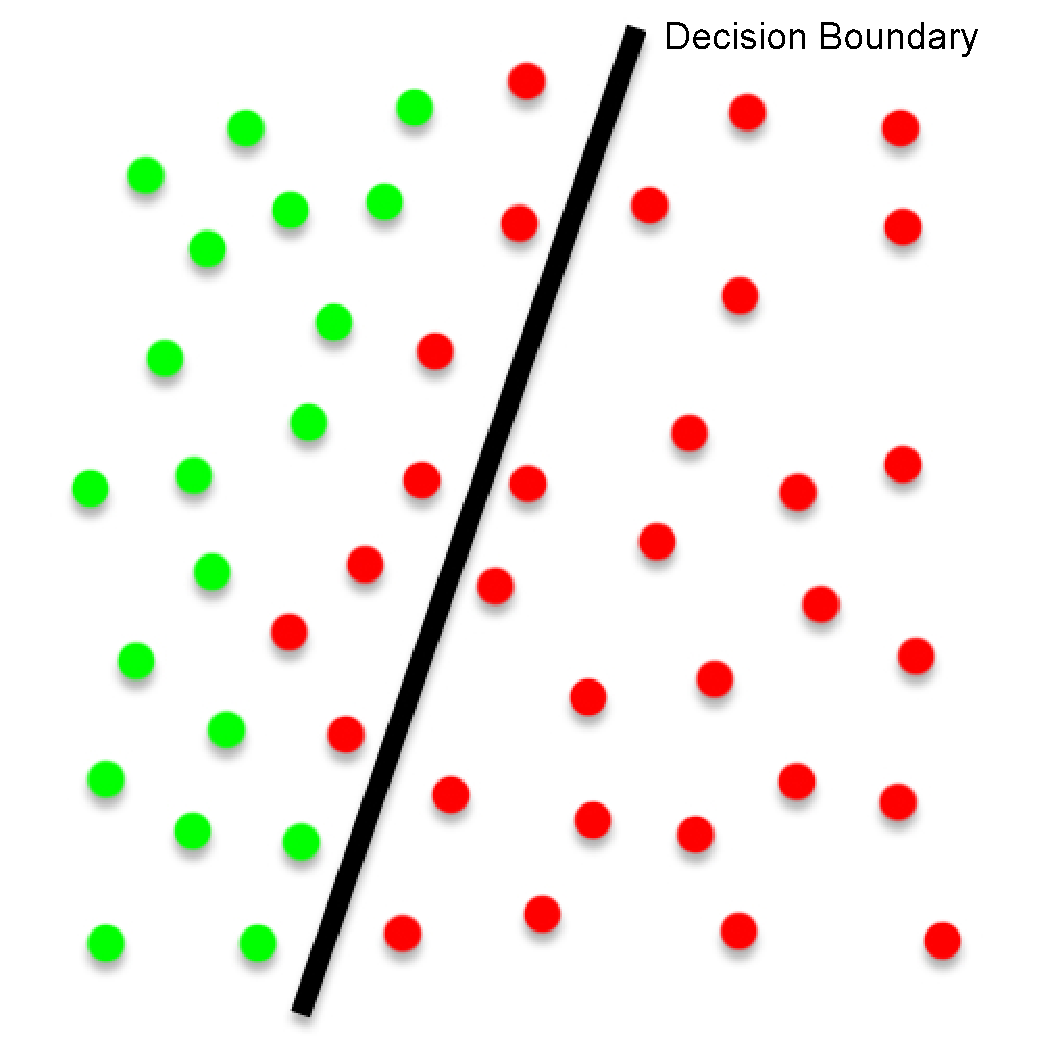
\includegraphics[width=0.5\linewidth]{Figures/Prune.pdf}
  \caption{Decision boundary created by classifier (illustrative purposes only.)}
  \label{fig:Prune}
\end{figure}
In Fig \ref{fig:Prune}, these classifiers create a decision boundary on the edges, where green edges are in the tour and red edges are not. Using repeated pruning, we can limit our data to edges that are part of the solution with few misclassified edges. After reducing the problem space, we can then execute an approximation algorithm on this smaller dataset, in turn providing close-to-optimal solution in significantly less time.

\section{Parameter Tuning}\label{parmeter_tuning}
\subsection{Sample Size}\label{sample-size}
As mentioned above in section \ref{pre-processing}, the training and testing sets comprised of 1000 nodes each. This was provided a lot of edge data as for each subgraph had $1000 \choose 2$ edges. It was also efficient for generating the ground truth as larger subgraphs would make it computationally in-effectient to generate the ground truth. \begin{figure}[h]
    \centering
  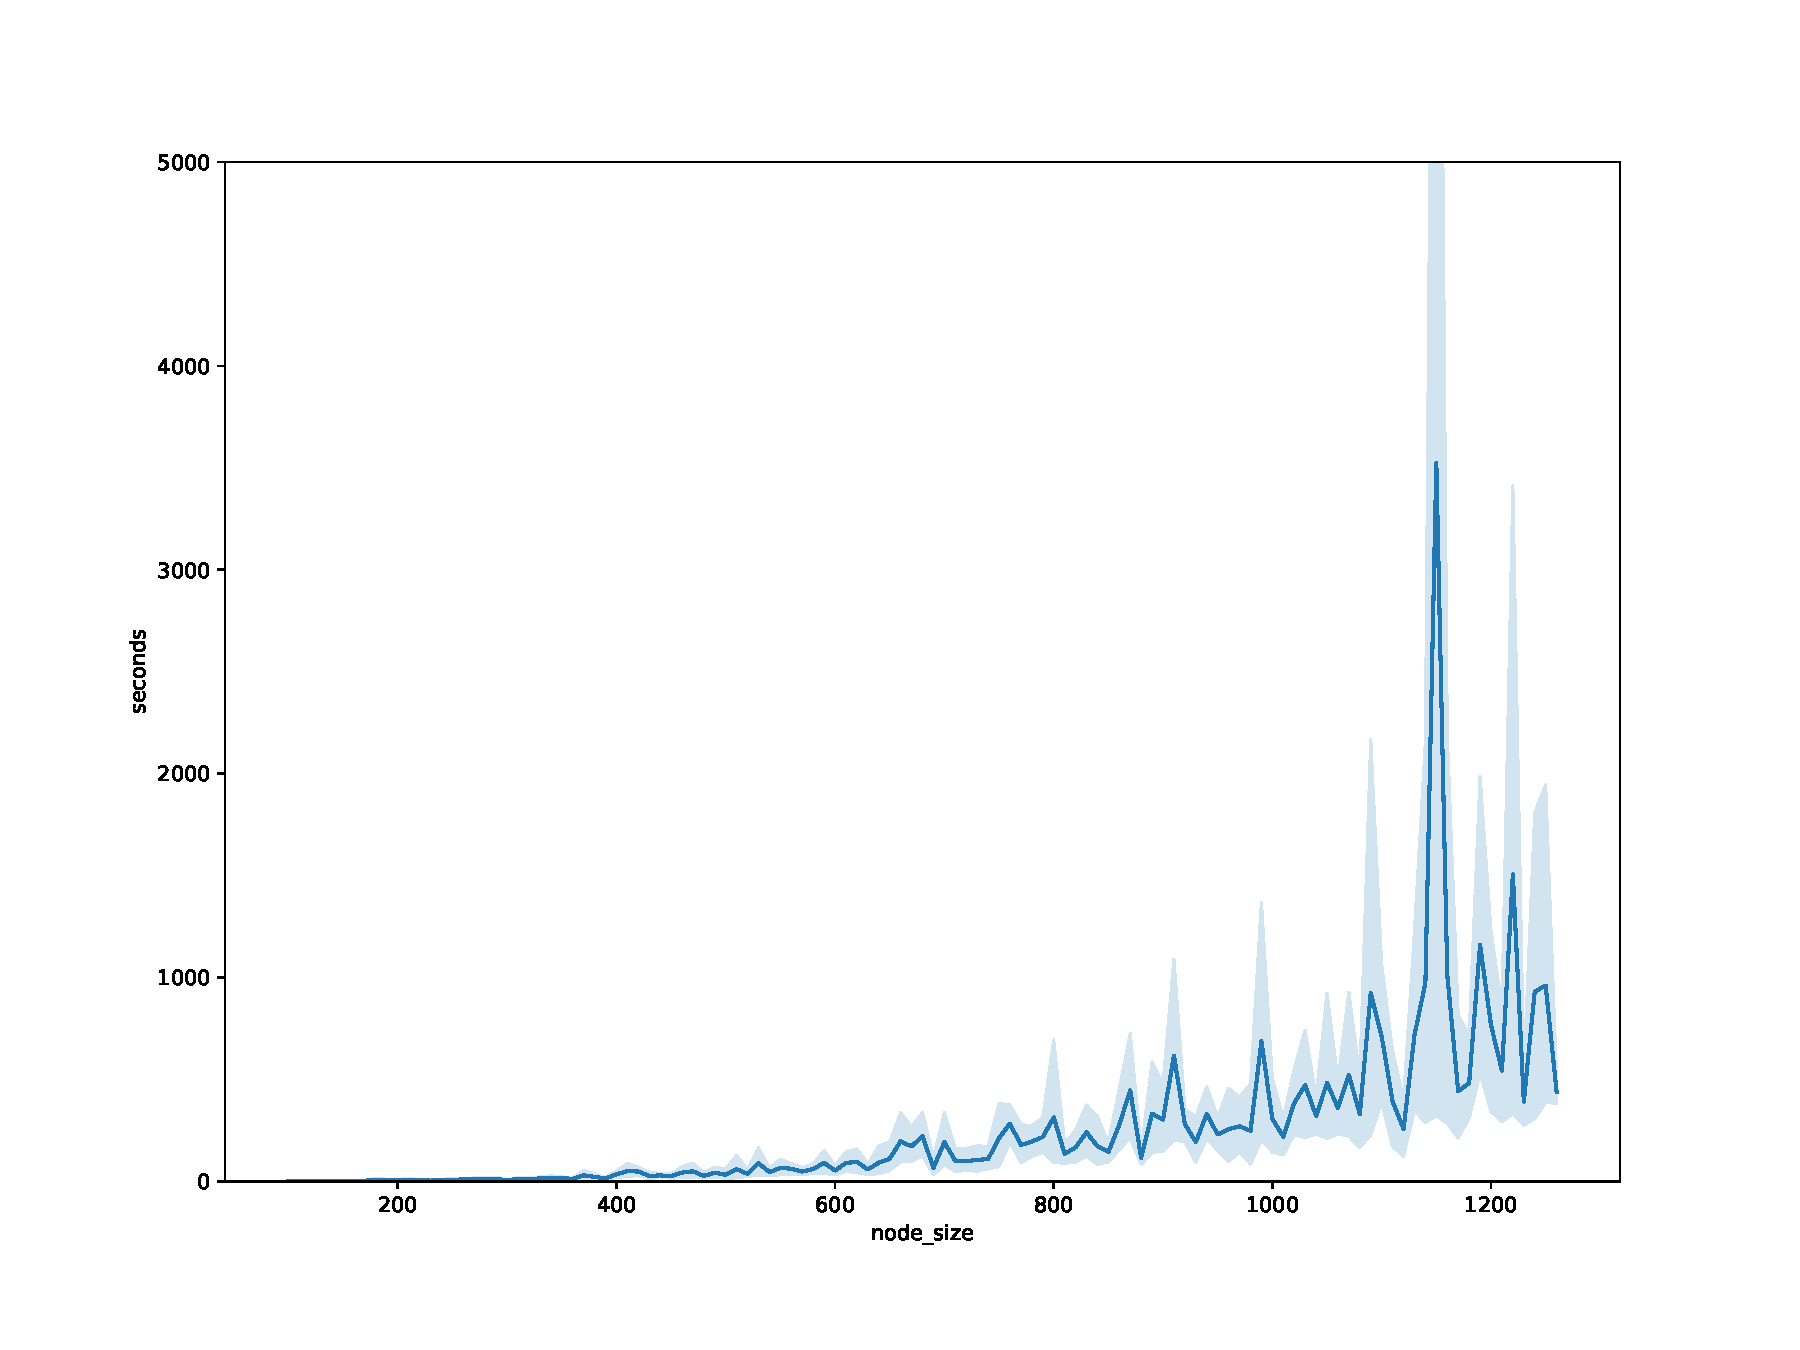
\includegraphics[width=1\linewidth]{Figures/runtime.pdf}
  \caption{Concorde running time as node input size increases}
  \label{fig:runtime}
\end{figure}

As seen in figure \ref{fig:runtime}, the running time tends to increase exponentially. Also as the number of nodes in the graph increases, the more chaotic the running times become.

\newpage
\subsection{Classifier Tuning}
Our main focus in this project was to use an ensamble approach like Random Forest to classify the edges that are containing in the TSP tour. The other two classifier that were training are used to compare against the Random Forest.
\begin{itemize}
    \item \textbf{Naïve Bayes Classifier: \newline}
        A Gaussian Naïve Bayes approach was used as our numeric data fit this classifier. This was used as a baseline to compare against the Random Forest Classifier.
    \item \textbf{Logistic Regression Classifier: \newline}
        This classifier was fit to the training data and was used to compare against the other Random Forest Classifier.
    \item \textbf{Random Forest Classifier: \newline}
        A grid search approach was used to find optimal parameters for this classifier. First a randomized search was performed on the parameter space. A localized search was performed on these results to fine tune this classifier.
\end{itemize}


%%%%%%%%

\chapter{Feature Engineering}\label{Feature_Engineering}
\section{Features used in training}
\begin{itemize}
    \item \textbf{Global Edge Rank: \newline}
        The global edge rank is defined as the number of edges that have a smaller weight (distance) than itself. A rank of 1 meaning that this is the smallest edge in the data.
    \item \textbf{Local Edge Rank: \newline}
        The local edge rank is computer incident to each edge of the nodes that make up an edge. This is similar to the Global rank, however the number of edges considered is in relation to a single node. These ranks range from 1 to $N-1$, as by definition of a complete graph, each node has $N-1$ edges incident to it.
    \item \textbf{Edge Statistics: \newline}
        These are Boolean variables that tell if an edge is within the 1st, 2nd or 3rd quartile.
    \item \textbf{Edge Weight: \newline}
        This is the distance between nodes given in kilometres. These were computed by the Concorde which uses a sphere approximation for the Earth as our data points are given in (latitude, longitude) pairs.
\end{itemize}

\section{Most important features}
These are features importance scores for the Random Forest model.
\begin{center}
\begin{tabular}{lr}
\toprule
\textbf{Feature Name} &  \textbf{Feature Importance Score} \\
\midrule
Local Rank Incident to Node2 &                  0.411630 \\
Local Rank Incident to Node1 &                  0.393103 \\
GLOBAL\_RANK                  &                  0.124089 \\
DISTANCE\_KM                  &                  0.069772 \\
IS\_IN\_1ST\_QUARTILE           &                  0.001231 \\
IS\_IN\_2ND\_QUARTILE           &                  0.000175 \\
IS\_IN\_3RD\_QUARTILE           &                  0.000000 \\
\bottomrule
\end{tabular}
\end{center}

As this is a combinatorial problem, it is unsurprising to see the local rankings provide more information than the edge weight itself.

\newpage
\section{Computational efficiency of features}
Global edge ranking was computed by sorting the entire list of edges by its weight and assigning a rank to each.

Local edge ranking required some pre-processing. A table of each node and its sorted list of corresponding incident edges was generated. This way sorting only needs to performed once whilst passing through every edge in the dataset. The local rank incident to a node was calculated by looking up the node in the table and find its target edge in the sorted list. Its rank would be corresponding to the position it had in this list.

The edge's quartiles were found by calculating the quartile boundaries and checking the edge's weight against those.

The edge weights were computed using the Concorde.

\chapter{Results}
\begin{figure}[!h]
   \centering
   \subfloat[Concorde Tour]{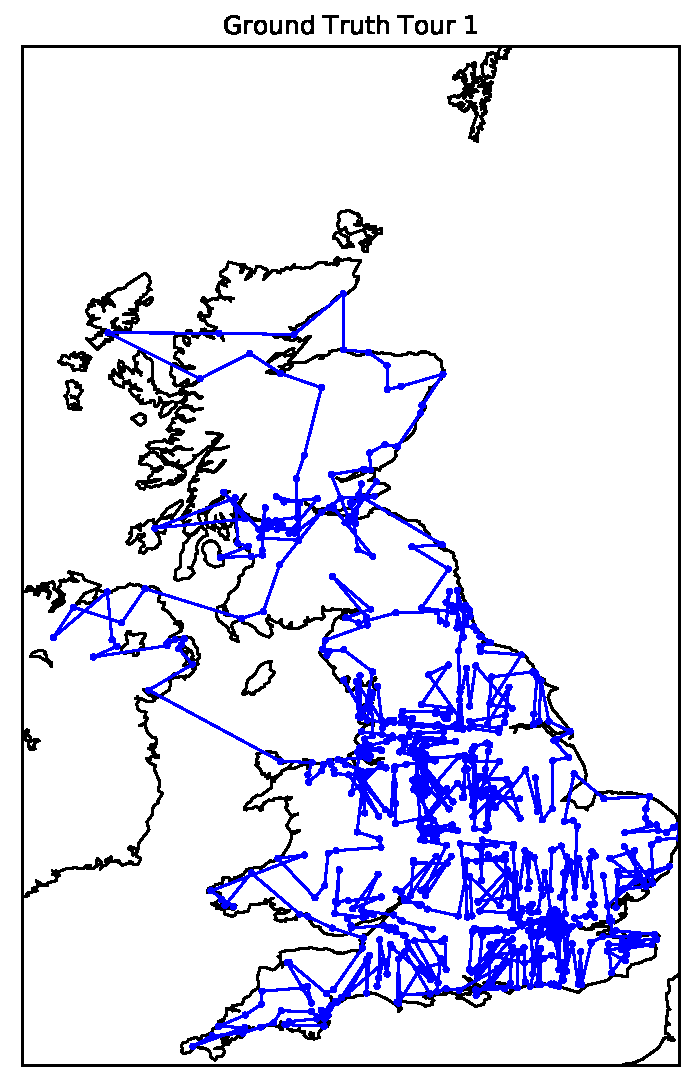
\includegraphics[width=0.4\textwidth]{Figures/map_plots/Ground Truth Tour 1.pdf}\label{fig:Concorde_tour}}
   \hfill
   \subfloat[Naïve Bayes Predicted Edges]{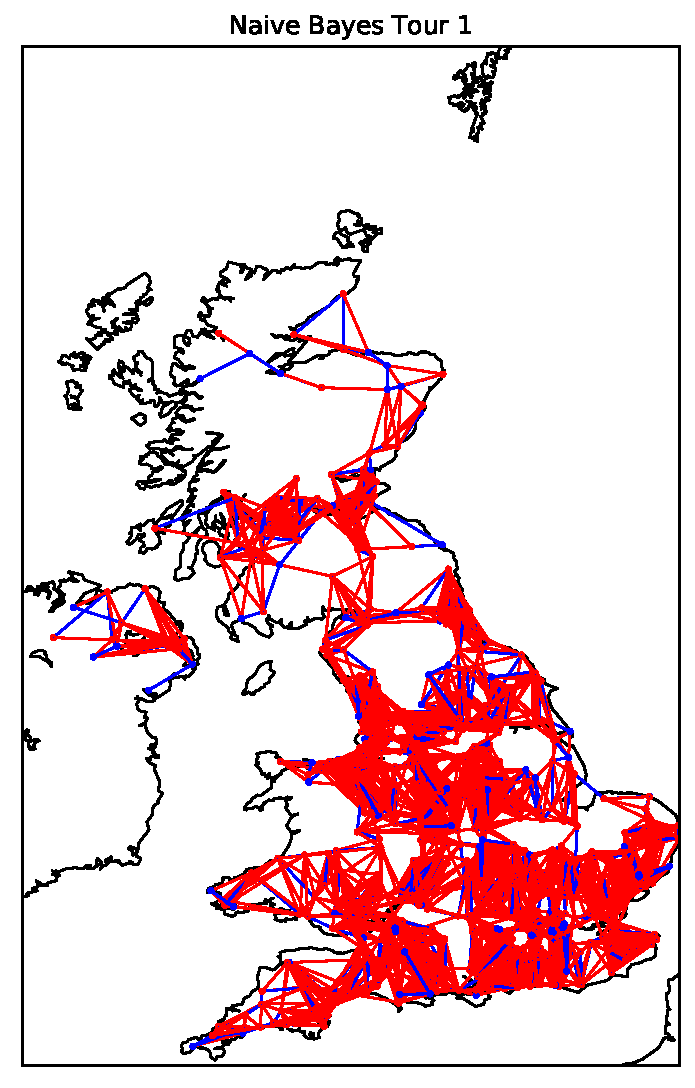
\includegraphics[width=0.4\textwidth]{Figures/map_plots/Naive Bayes Tour 1.pdf}\label{fig:NB_tour}}
   \hfill
   \subfloat[Logistic Regression Predicted Edges]{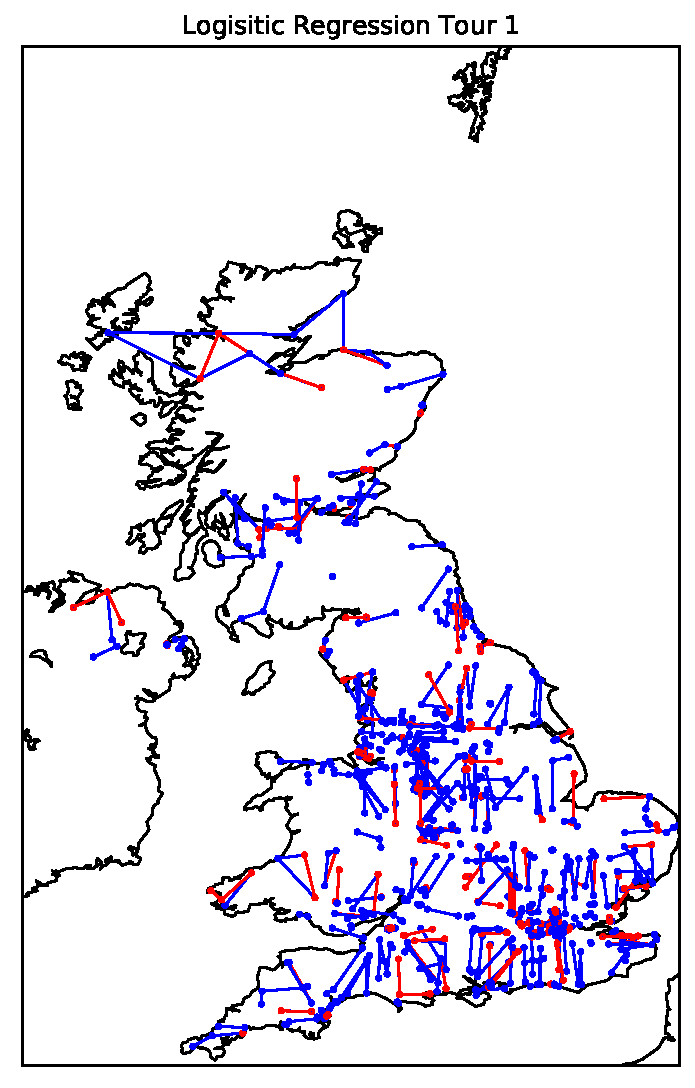
\includegraphics[width=0.4\textwidth]{Figures/map_plots/Logisitic Regression Tour 1.pdf}\label{fig:LR_tour}}
   \hfill
   \subfloat[Random Forest Predicted Edges]{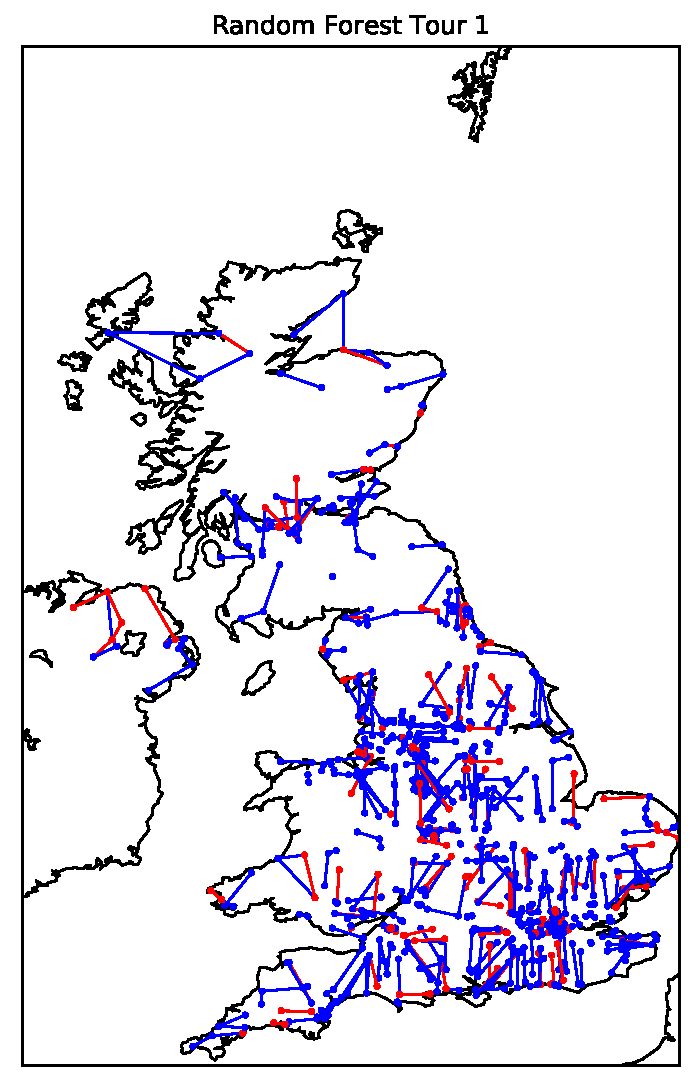
\includegraphics[width=0.4\textwidth]{Figures/map_plots/Random Forest Tour 1.pdf}\label{fig:RF_tour}}
  \caption{Concorde vs. Classifier Predicted Edges}
\end{figure}\label{fig:concorde vs. classifiers}

To put our results into context, we must look at the tour generated by the Concorde and compare it against the edges that our models predicted. The number in the titles correspond to graph in the test set. Blue edges represent edges that are contained in the ground truth and red edges are edges predicted by the classifier that were not in the ground truth.

Naïve Bayes performed very poorly, it predicted a large amount of edges that were not in the ground truth, this can be clearly seen in Fig \ref{fig:concorde vs. classifiers}. This discovery is further enforced by its extremely low f1-score of 0.22. However, as it predicts so many edges, it tends to keep a lot of the ground truth in its predictions, this fact is backed up by its recall score of 0.99. A different picture is painted when comparing the Logistic regression and Random forest classifiers. From plotting their predicted edges, we can see very similar results. This is an unexpected discovery as the Random forest classifier has a more complex structure. Both classifiers share similar f1-score around 0.66.

Logistic regression and Random forest both remove a significant amount of the ground truth’s edges whilst Naïve Bayes predicts too many edges. We try to amend this issue by introducing a threshold value. Each edge has a prediction probability, in the above figures (\ref{fig:concorde vs. classifiers}), the threshold is set at a default of 0.5, meaning that any edge with a probability of less than 50\% will not be predicted. However, by adjusting this threshold value we can choose to include more edges by reducing it.

Results for other test graphs can be seen in section \ref{addendum_1}

\newpage
\textbf{Thresholding}
\begin{figure}[!h]
    \centering
    \subfloat[Naïve Bayes]{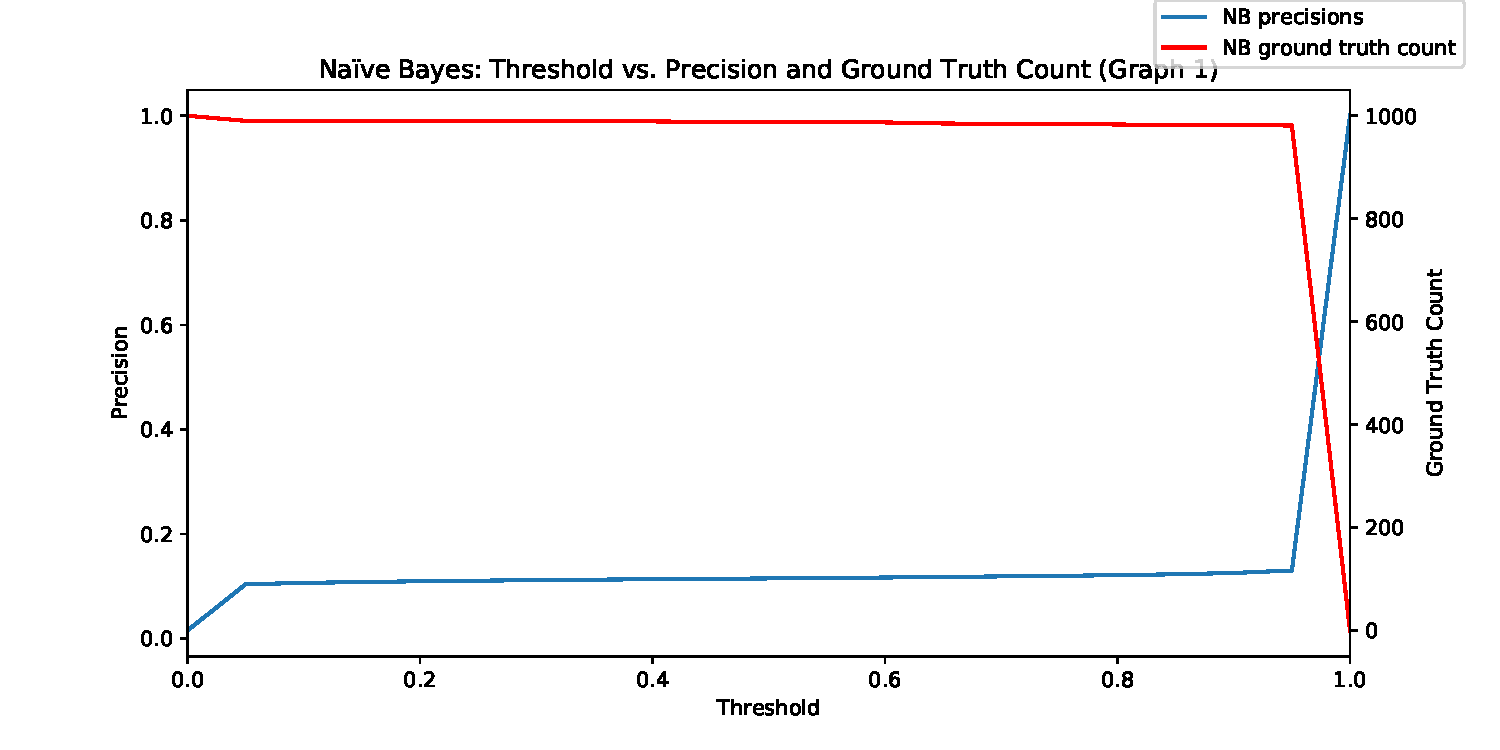
\includegraphics[width=0.8\textwidth]{Figures/exp1/NB thresh vs. precision and gtruth 1.pdf}\label{fig:NB_thresh}}
    \hfill
    \subfloat[Logistic Regression]{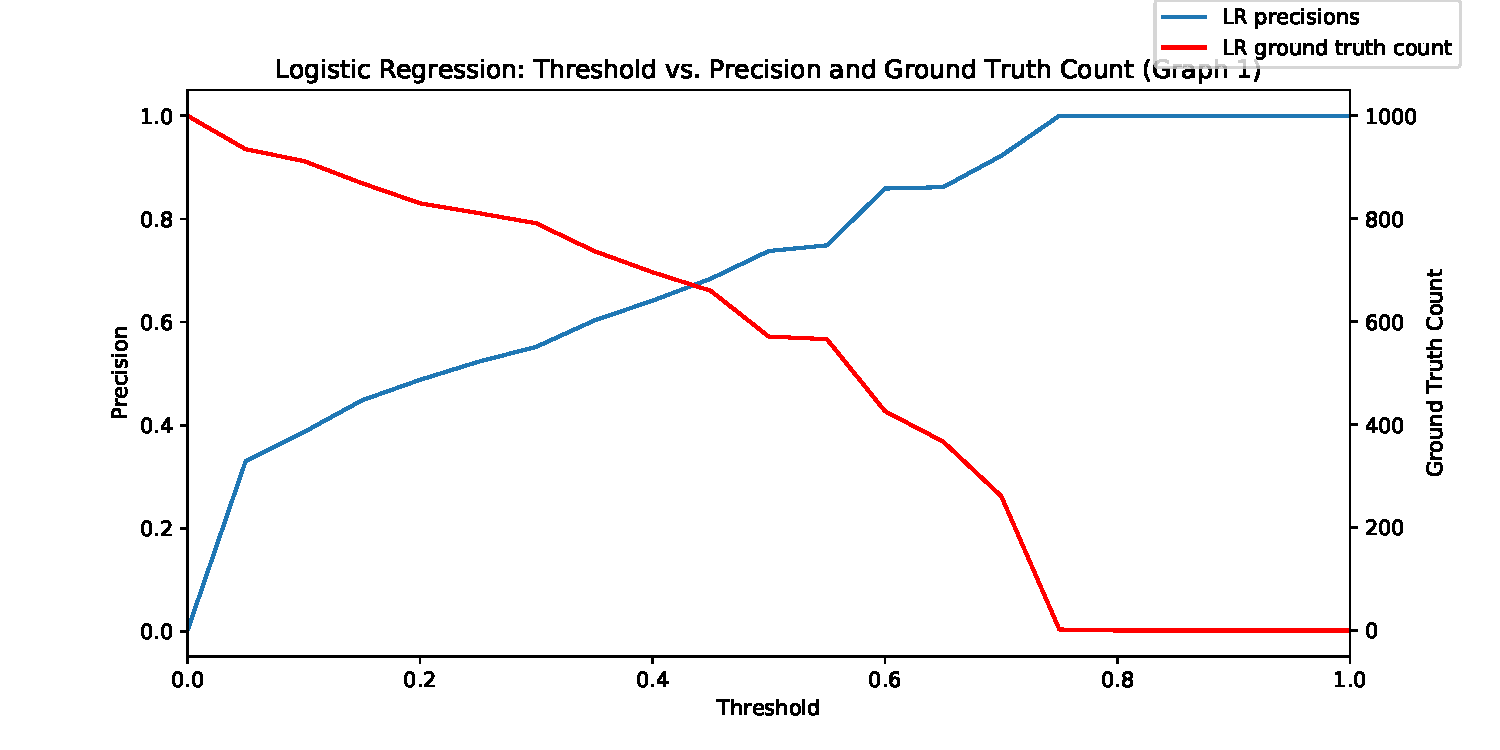
\includegraphics[width=0.8\textwidth]{Figures/exp1/LR thresh vs. precision and gtruth 1.pdf}\label{fig:LR_thresh}}
    \hfill
    \subfloat[Random Forest]{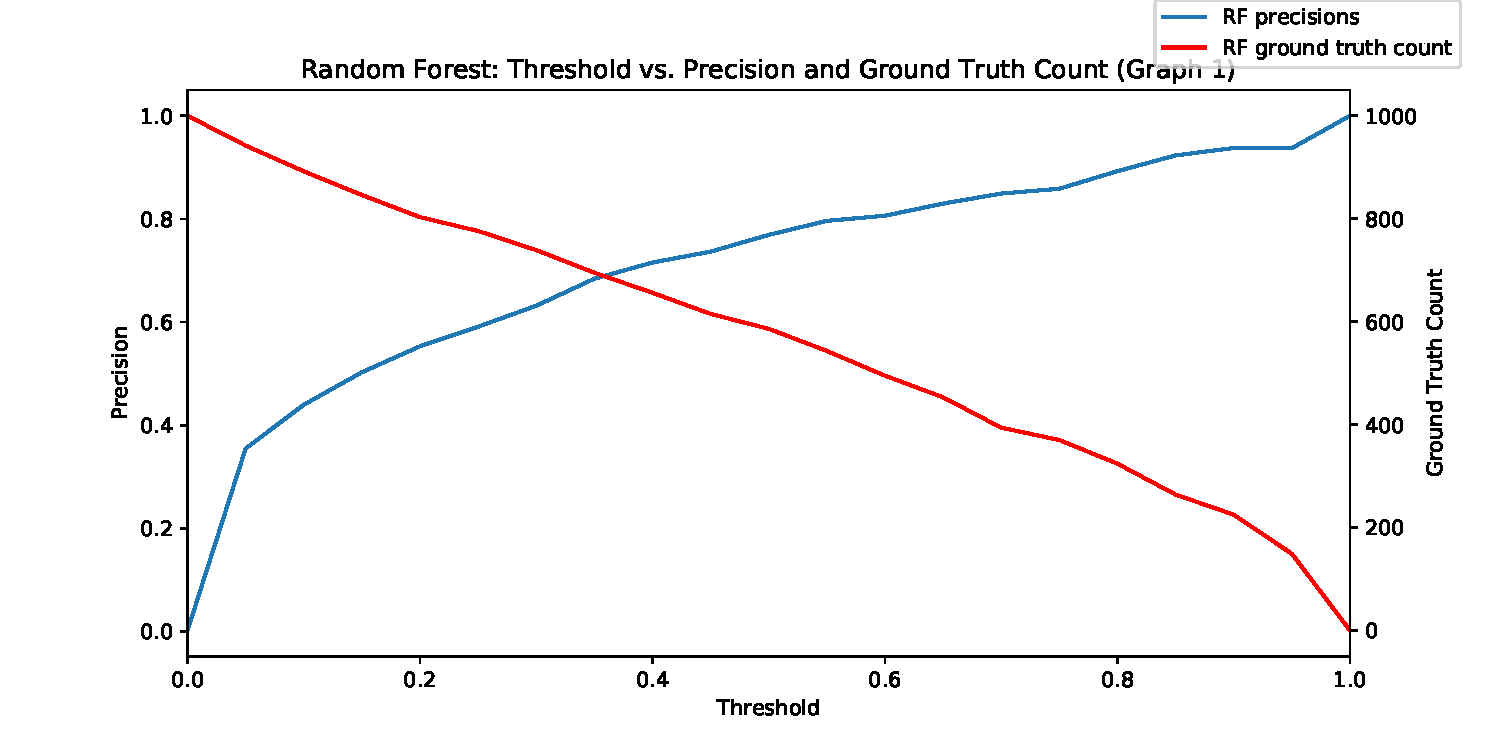
\includegraphics[width=0.8\textwidth]{Figures/exp1/RF thresh vs. precision and gtruth 1.pdf}\label{fig:RF_thresh}}
    \caption{Adjusting Threshold Values}
\end{figure}\label{fig:Classifiers vs. Threshold}

\newpage
Adjusting the threshold value allows us to fine tune how many edges we prune from our initial edge dataset. Naïve Bayes responded poorly to the threshold testing as the precision stays very low throughout most of the threshold values. We see a sudden spike in precision towards the higher threshold values, this is because most of the edges have been pruned, and the sample size is far too small to draw any reasonable conclusions. Logistic regression has a steady increase in precision as we increase the threshold values. Ideally, we would like the precision to start higher and plateau sooner for optimal pruning. A similar conclusion can be drawn from the Random forest testing however the scores and ground truth count transition smoothly between different threshold values.

More results for other test graphs can be seen in section \ref{addendum_2}

\textbf{Non-Pruning Ratio vs. Precision}

The prune ratio is defined as the following:

\begin{equation*}
    \text{Prune Ratio} = 1 - \frac{\# \text{Predicted Edges}}{\# \text{Total Edges}}
\end{equation*}

\begin{equation*}
    \text{Non-Pruning Ratio} = 1 - \text{Prune Ratio}
\end{equation*}

A pruning ratio of 1 corresponds to classifier removing every edge and a ratio of 0 means that the classifier predicts every edge possible. It is the ratio of how many edges are removed by the classifier. Of course, this value changes depending on the threshold value. The Non-pruning ratio would be 1 – Prune Ratio, showing us the ratio of edges we keep. Examining the Non-pruning ratio vs. Precision curve for each classifier can help us find the optimal threshold value.

\begin{figure}[!h]
    \centering
    \subfloat[Naïve Bayes]{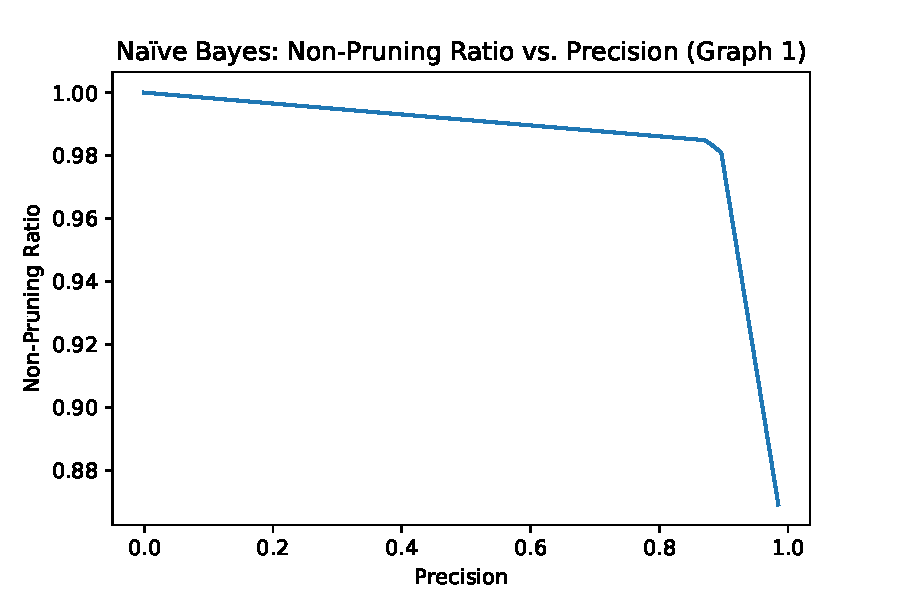
\includegraphics[width=0.7\textwidth]{Figures/exp2/NB non-prune vs precision 1.pdf}\label{fig:NB_nonprune_vs_precision}}
    \hfill
    \subfloat[Logistic Regression]{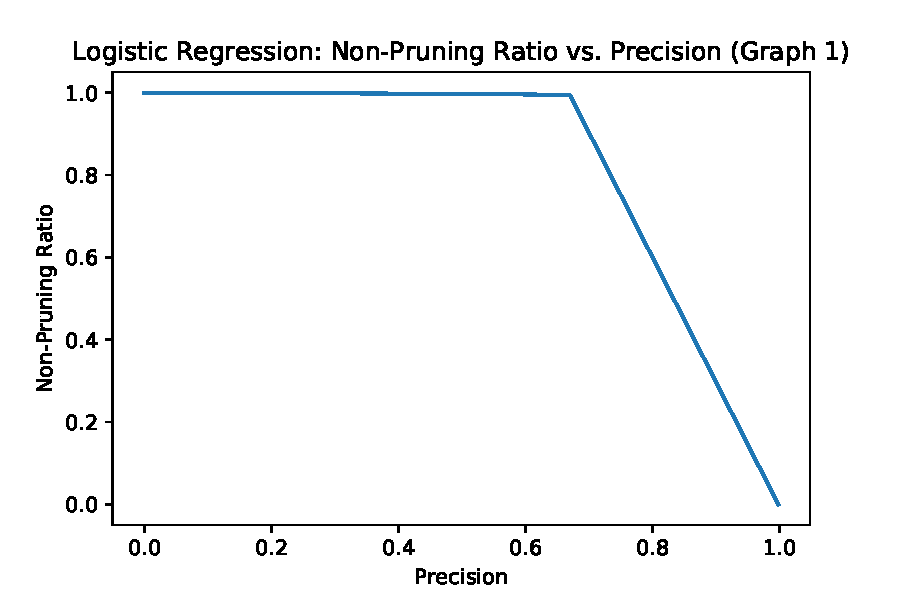
\includegraphics[width=0.7\textwidth]{Figures/exp2/LR non-prune vs precision 1.pdf}\label{fig:LR_nonprune_vs_precision}}
    \hfill
    \subfloat[Random Forest]{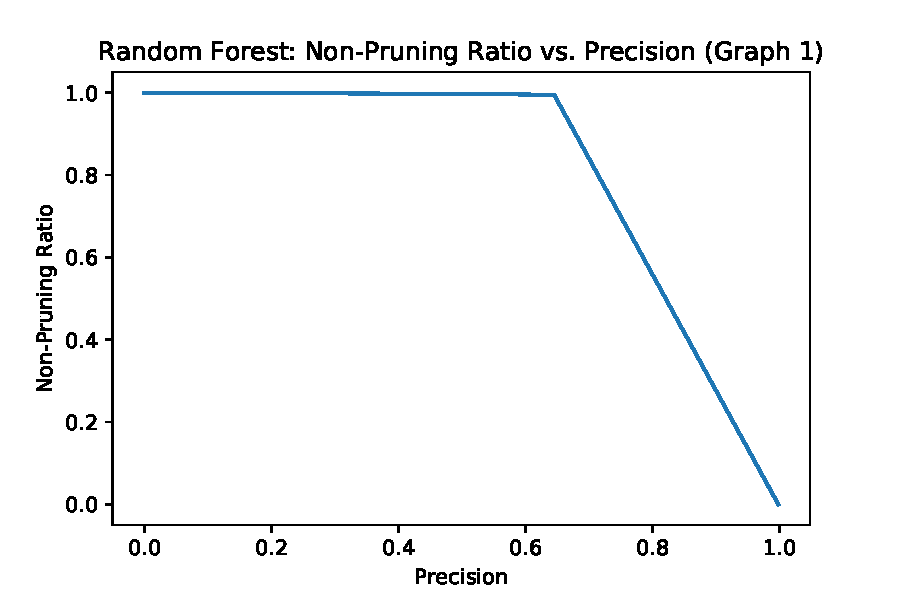
\includegraphics[width=0.7\textwidth]{Figures/exp2/RF non-prune vs precision 1.pdf}\label{fig:RF_nonprune_vs_precision}}
    \caption{Non-pruning ratio vs. Precision curve}
\end{figure}\label{fig:non-prune vs precision}

The most optimal threshold can be found by looking at the pair of Non-pruning and precision values at the point on the curve just before values drop. Naïve Bayes does not remove enough edges, at its optimal point, slightly less than 2\% of the edges have been pruned. Logistic regression and Random forest perform similarly. Their optimal thresholds also do not yield a high enough precision. Going further along the curve, increasing the precision, we risk over pruning which could remove ground truth edges. These results can be seen in Figure \ref{fig:non-prune vs precision}.

Results for other tests graphs can be found in section \ref{addendum_3}.



%%%%%%%%
\chapter{Conclusion and Future Work}
\section{Conclusion}
Combinatorial optimization is an NP-Hard problem that has many applications. In this thesis, we considered the travelling salesman problem (TSP), one of the classical combinatorial optimization problems. We reviewed the various techniques to solve the TSP from exact algorithms to complex Deep Learning frameworks. We used machine learning classification frameworks to identify the edges in the TSP tour. This prediction was then used to prune edges that are not in a TSP tour, that then enables us to scale-up exact and approximation algorithms. We were able to prune a small percentage of edges that weren't in the TSP solution. This small set of pruned edges is not a satisfiable result and future work is required (Sec. \ref{section: future work}).

All code and is publicly available on GitHub \href{https://github.com/SabeerBakir/Learning-shortest-path-tours-to-all-pubs-in-UK}{here}.


\section{Future Work}\label{section: future work}
\begin{itemize}
    \item Implementing the time taken to travel from node to node instead of distance as a metric for increased accuracy to the solution, using the Google Maps API.
    \item Training these models on other datasets, for example, pubs in other countries, datasets for delivery/postal service scenarios. 
    \item Integrate an exact algorithm such as Held-Karp algorithm \cite{Bellman:1962:DPT:321105.321111}.
    \item Perform further feature engineering to better characterise edges in the dataset.
\end{itemize}



%%%%%%%%%%%%%%%%%%%%%%
%%%% Latex help.
%\chapter{Latex Pointers}

This chapter contains some examples on the usage of latex. Do not include in your final report.

\section{Figures}
From time to time, it's necessary to add pictures to your documents. Using LaTeX all pictures will be indexed automatically and tagged with successive numbers when using the figure environment and the graphicx package. We can reference the figure below using its label like this: Fig. \ref{fig:test_plot}.
\begin{figure}[h]
    \centering
  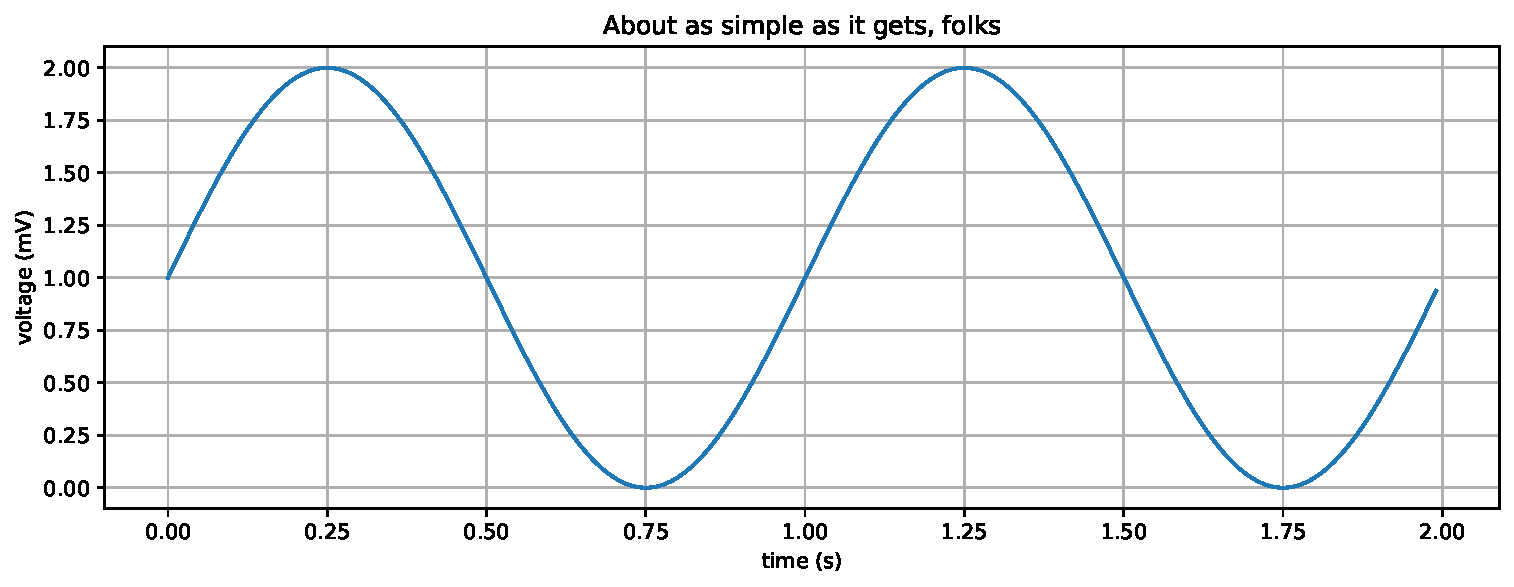
\includegraphics[width=0.8\linewidth]{test_plot.pdf}
  \caption{A sample graph}
  \label{fig:test_plot}
\end{figure}

Lots more information in this \href{https://www.latex-tutorial.com/tutorials/figures/}{tutorial}.


\section{Code Listing}
You can list code using the \emph{listings} package:

\begin{lstlisting}[language=Python,caption=Borg Pattern]
class Borg(object):
    __shared_state = {}

    def __init__(self):
        self.__dict__ = self.__shared_state
        self.state = 'Init'

    def __str__(self):
        return self.state
\end{lstlisting}

Lots more examples \href{https://www.overleaf.com/learn/latex/Code_listing}{here}.

\section{Math}
Here \ref{eq:limit} is an example of including an equation
\begin{equation}
\lim_{x\to\infty} f(x)
\label{eq:limit}
\end{equation}

More examples \href{https://www.latex-tutorial.com/tutorials/amsmath/}{here} and \href{https://www.overleaf.com/learn/latex/Mathematical_expressions}{here}.



\section{References}
Look up the bibtex references on google scholar or import from Mendeley or other reference managers. Add the bibtex snippet to the \emph{references.bib} file. Then cite the reference like this:

As explained in \cite{knuth2014art}, we also find that...

Lots more details \href{https://www.latex-tutorial.com/tutorials/bibtex/}{here}.


%%%%%%%%%%%%%%%%%%%%%%
%%% Acknowledgements
\chapter*{Acknowledgements}
I would like to thank University College Dublin’s school of Computer Science for their support and Dr. Deepak Ajwani for his guidance throughout this project.

\chapter{Addendum}
\section{Addendum 1}\label{addendum_1}
\begin{figure}[!h]
   \centering
   \subfloat[Concorde Tour]{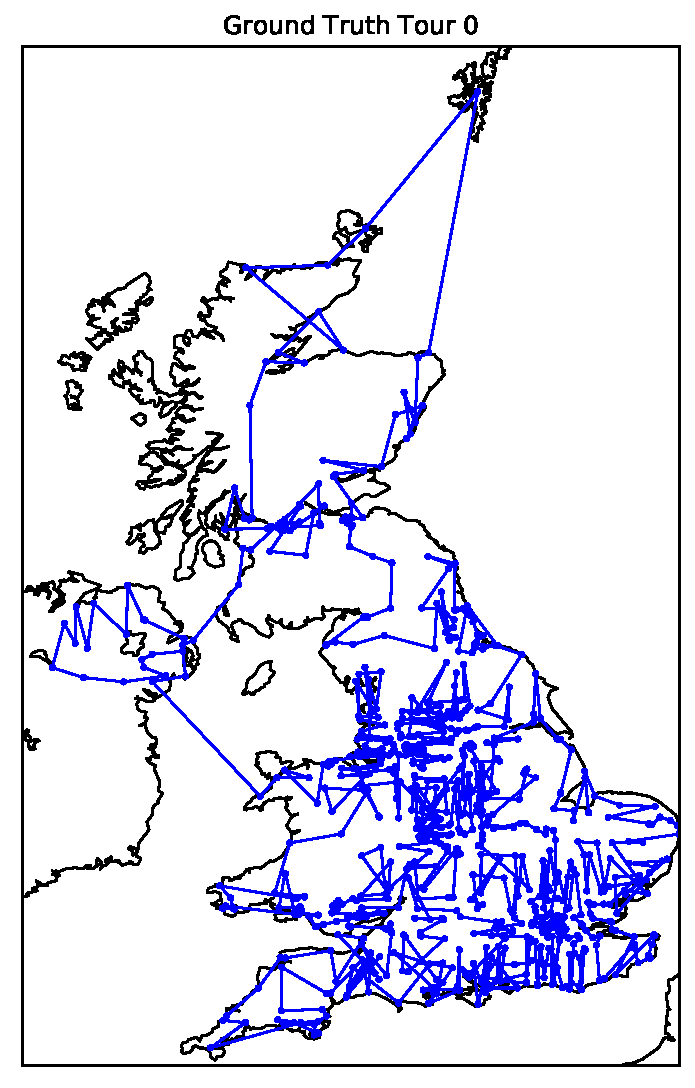
\includegraphics[width=0.35\textwidth]{Figures/map_plots/Ground Truth Tour 0.pdf}}
   \hfill
   \subfloat[Naïve Bayes Predicted Edges]{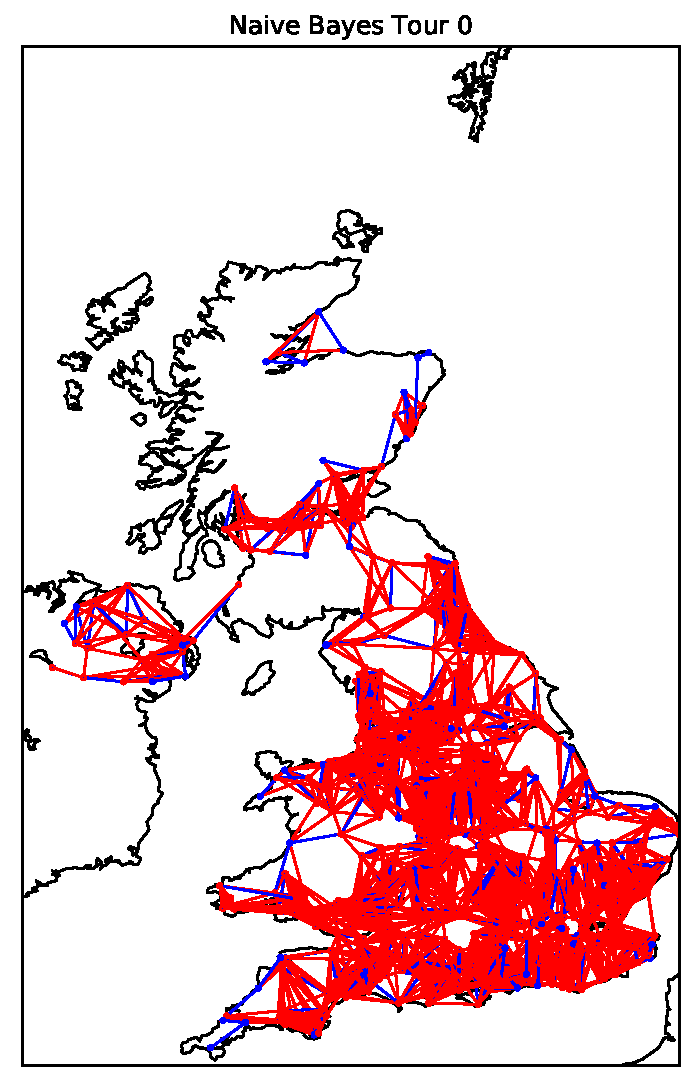
\includegraphics[width=0.35\textwidth]{Figures/map_plots/Naive Bayes Tour 0.pdf}}
   \hfill
   \subfloat[Logistic Regression Predicted Edges]{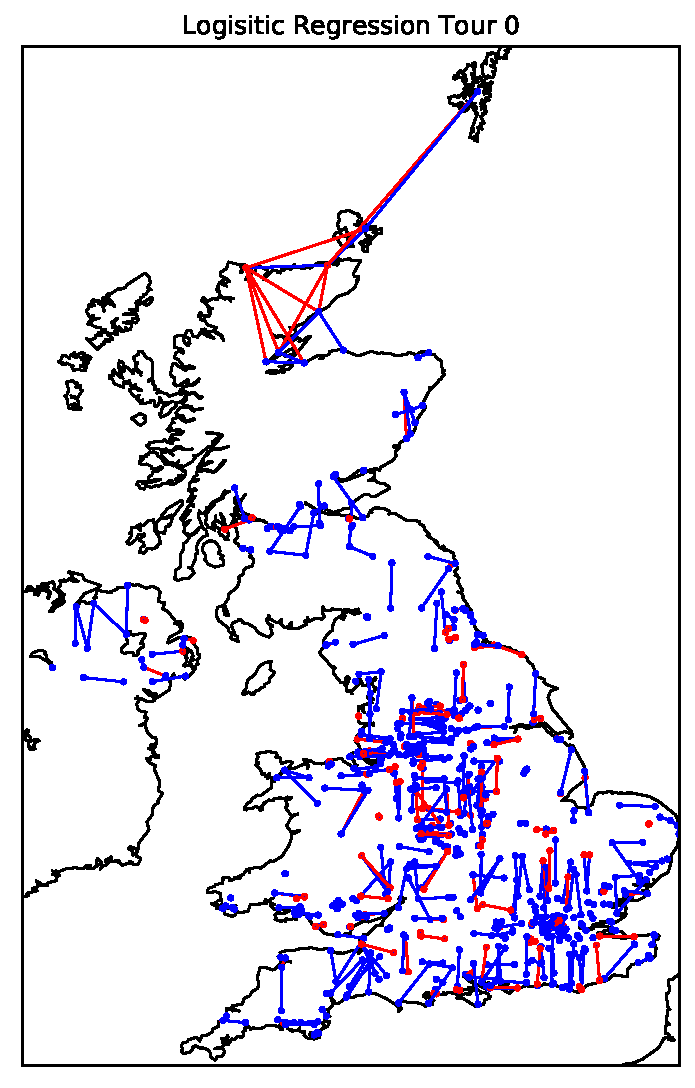
\includegraphics[width=0.35\textwidth]{Figures/map_plots/Logisitic Regression Tour 0.pdf}}
   \hfill
   \subfloat[Random Forest Predicted Edges]{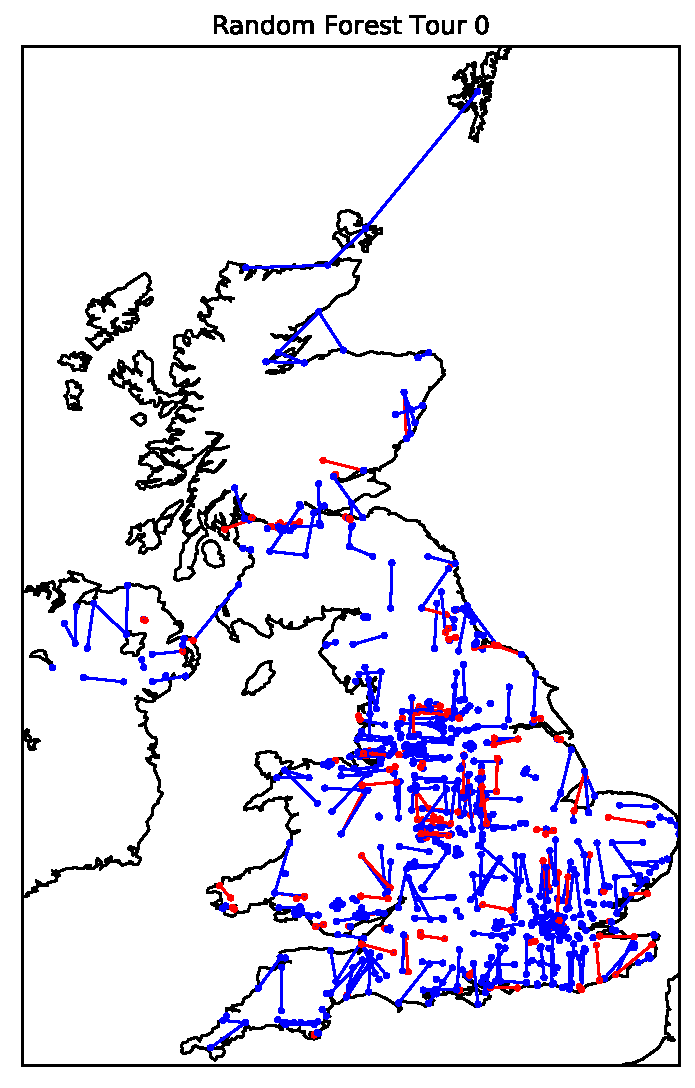
\includegraphics[width=0.35\textwidth]{Figures/map_plots/Random Forest Tour 0.pdf}}
  \caption{Concorde vs. Classifier Predicted Edges}
\end{figure}

\begin{figure}[!h]
   \centering
   \subfloat[Concorde Tour]{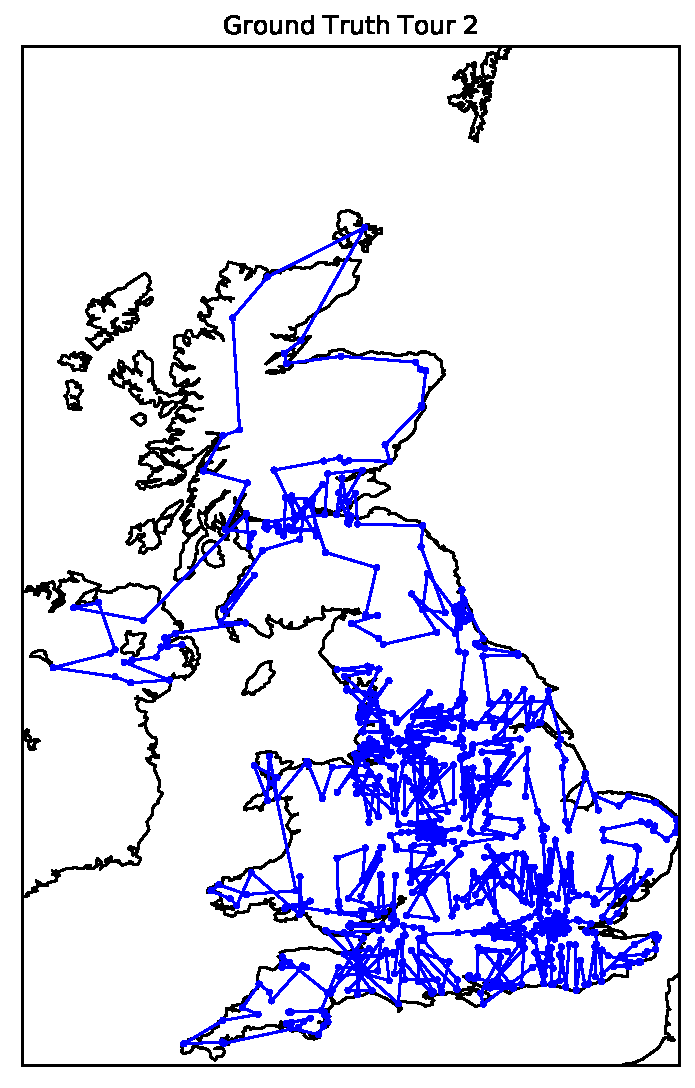
\includegraphics[width=0.4\textwidth]{Figures/map_plots/Ground Truth Tour 2.pdf}}
   \hfill
   \subfloat[Naïve Bayes Predicted Edges]{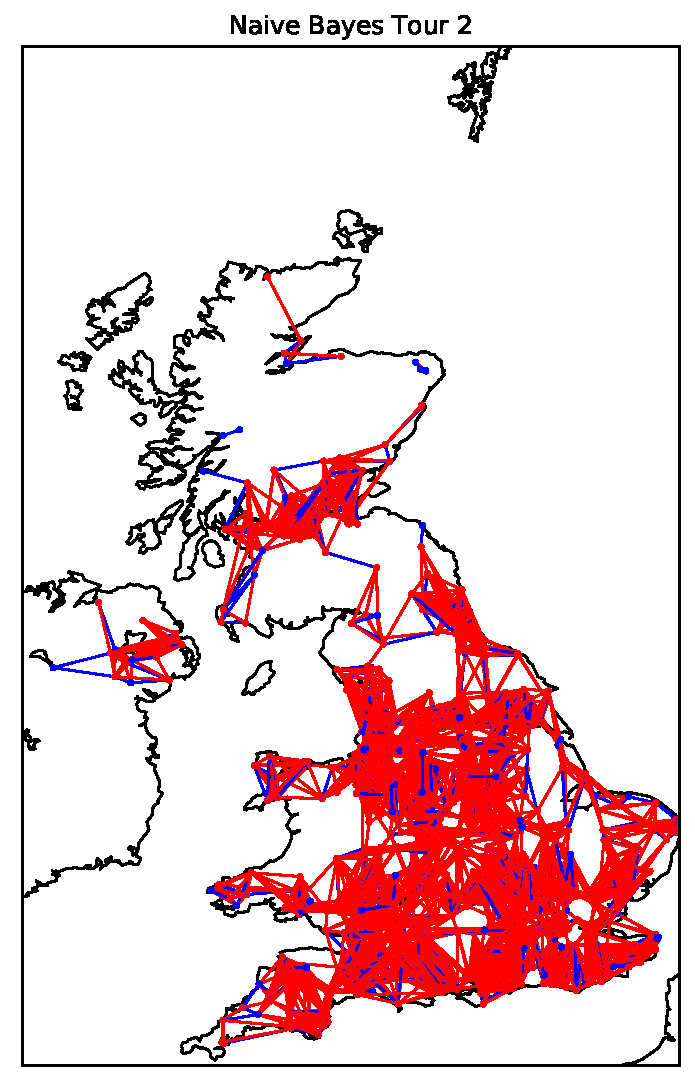
\includegraphics[width=0.4\textwidth]{Figures/map_plots/Naive Bayes Tour 2.pdf}}
   \hfill
   \subfloat[Logistic Regression Predicted Edges]{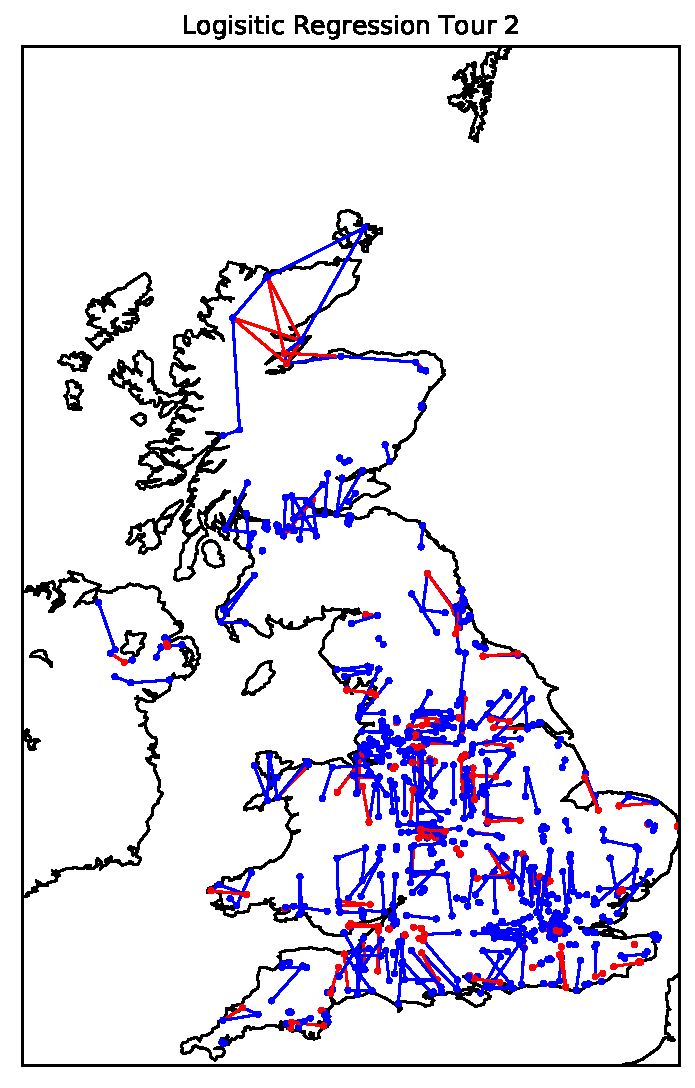
\includegraphics[width=0.4\textwidth]{Figures/map_plots/Logisitic Regression Tour 2.pdf}}
   \hfill
   \subfloat[Random Forest Predicted Edges]{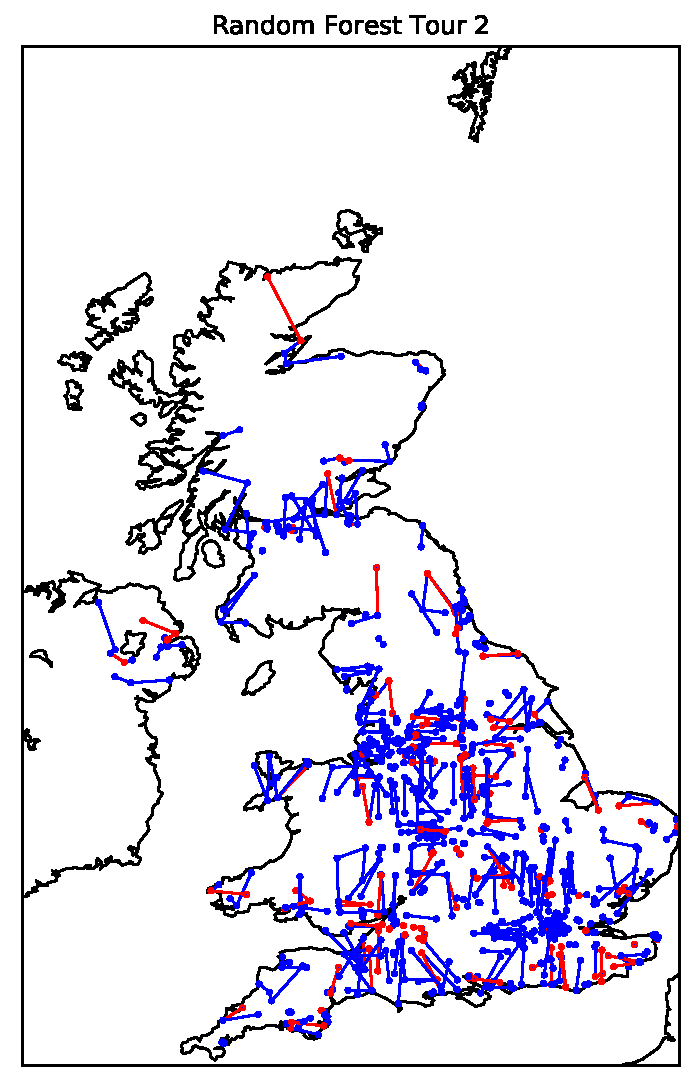
\includegraphics[width=0.4\textwidth]{Figures/map_plots/Random Forest Tour 2.pdf}}
  \caption{Concorde vs. Classifier Predicted Edges}
\end{figure}

\begin{figure}[!h]
   \centering
   \subfloat[Concorde Tour]{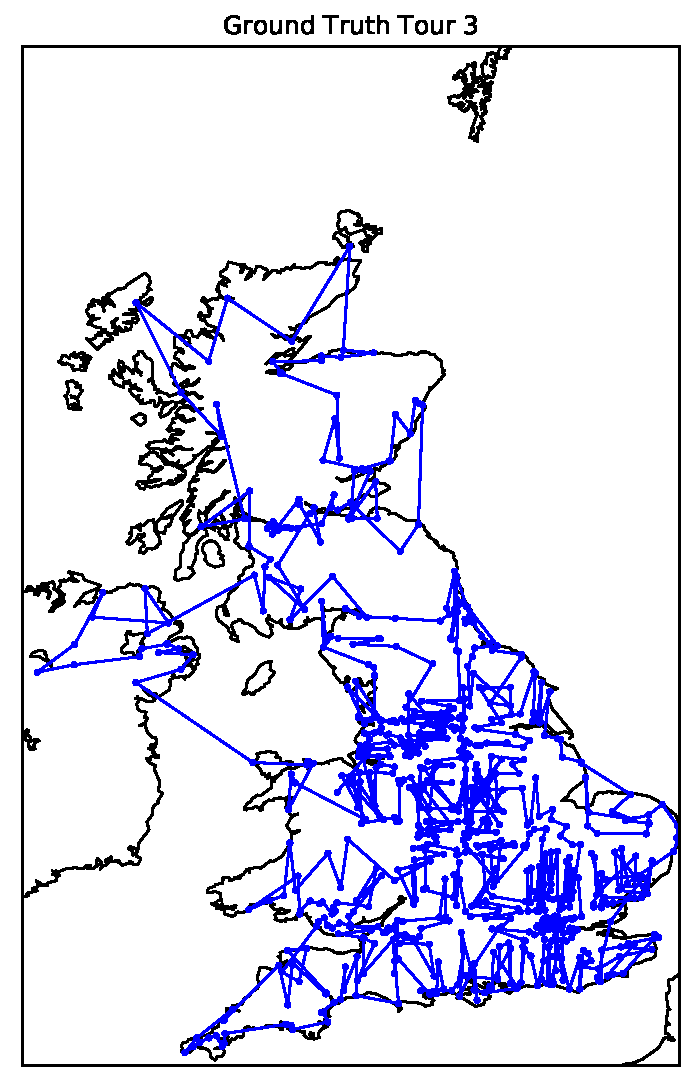
\includegraphics[width=0.4\textwidth]{Figures/map_plots/Ground Truth Tour 3.pdf}}
   \hfill
   \subfloat[Naïve Bayes Predicted Edges]{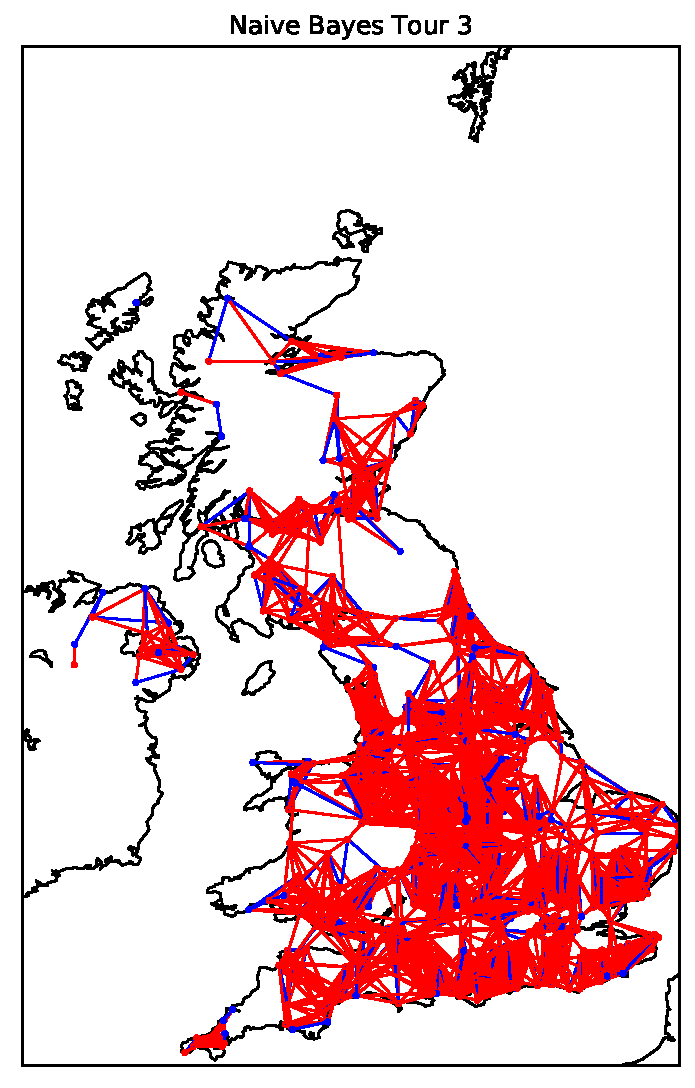
\includegraphics[width=0.4\textwidth]{Figures/map_plots/Naive Bayes Tour 3.pdf}}
   \hfill
   \subfloat[Logistic Regression Predicted Edges]{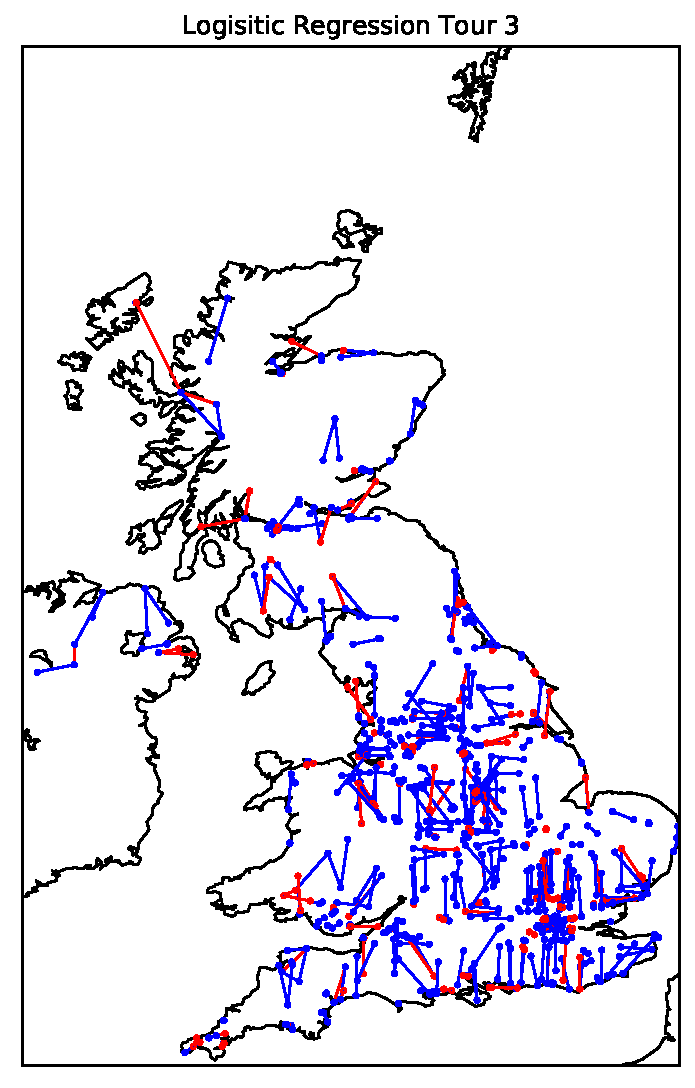
\includegraphics[width=0.4\textwidth]{Figures/map_plots/Logisitic Regression Tour 3.pdf}}
   \hfill
   \subfloat[Random Forest Predicted Edges]{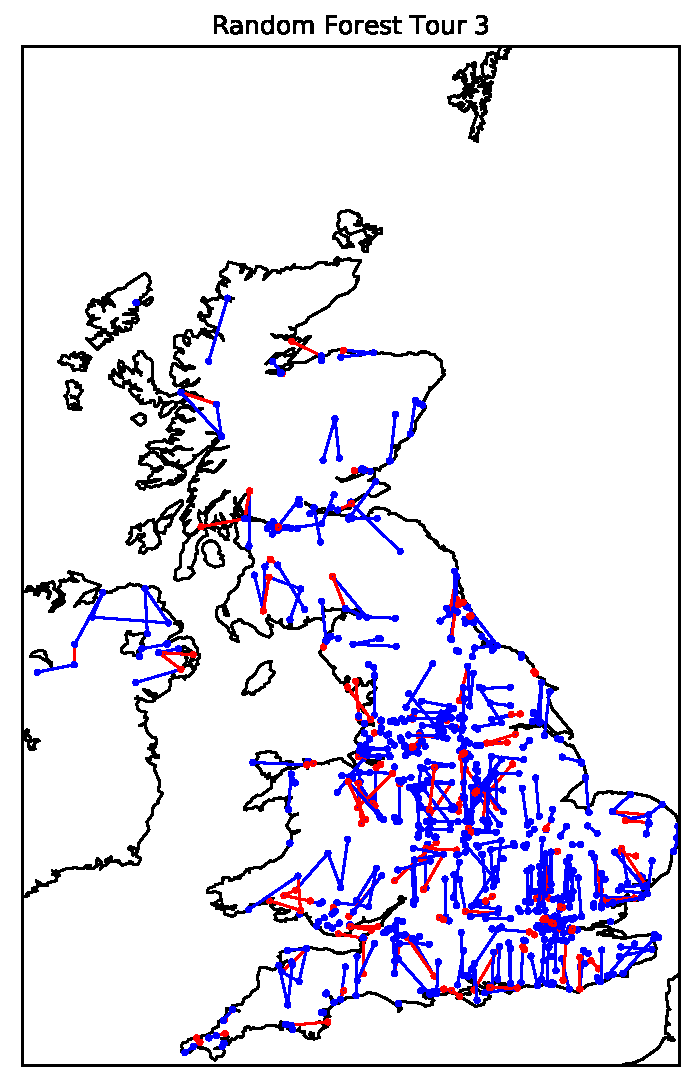
\includegraphics[width=0.4\textwidth]{Figures/map_plots/Random Forest Tour 3.pdf}}
  \caption{Concorde vs. Classifier Predicted Edges}
\end{figure}

\begin{figure}[!h]
   \centering
   \subfloat[Concorde Tour]{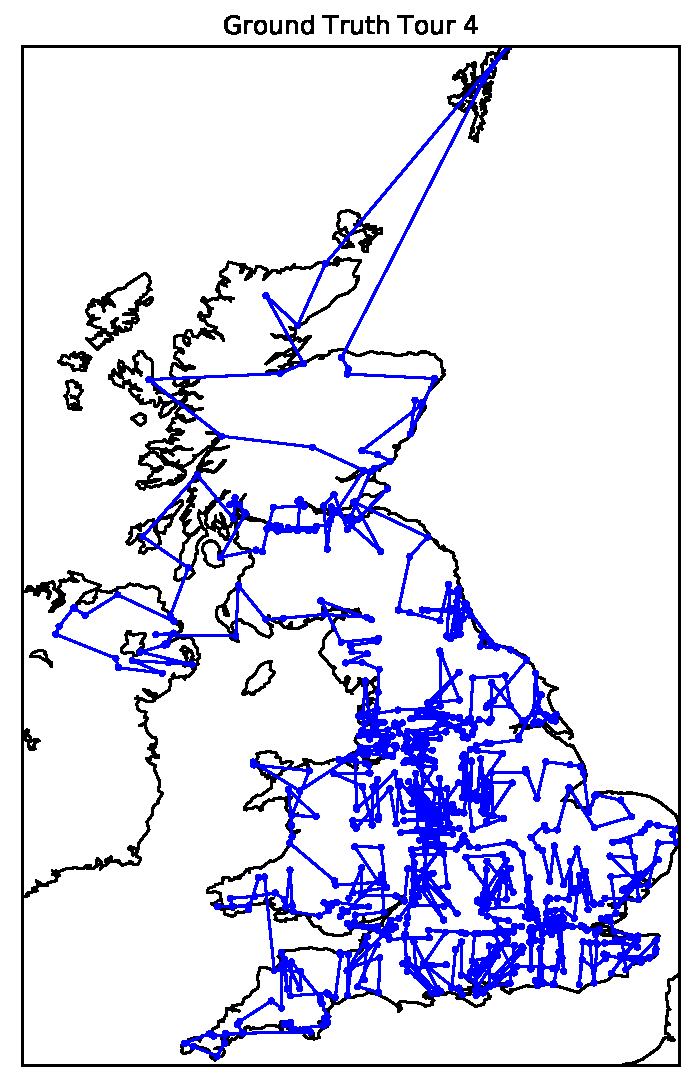
\includegraphics[width=0.4\textwidth]{Figures/map_plots/Ground Truth Tour 4.pdf}}
   \hfill
   \subfloat[Naïve Bayes Predicted Edges]{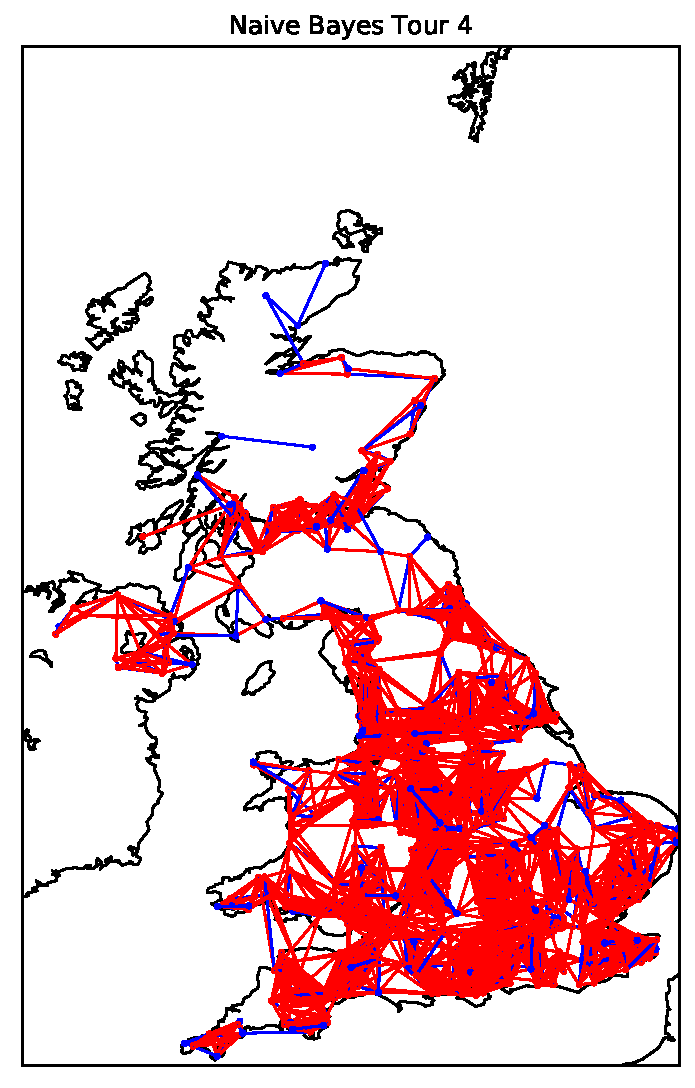
\includegraphics[width=0.4\textwidth]{Figures/map_plots/Naive Bayes Tour 4.pdf}}
   \hfill
   \subfloat[Logistic Regression Predicted Edges]{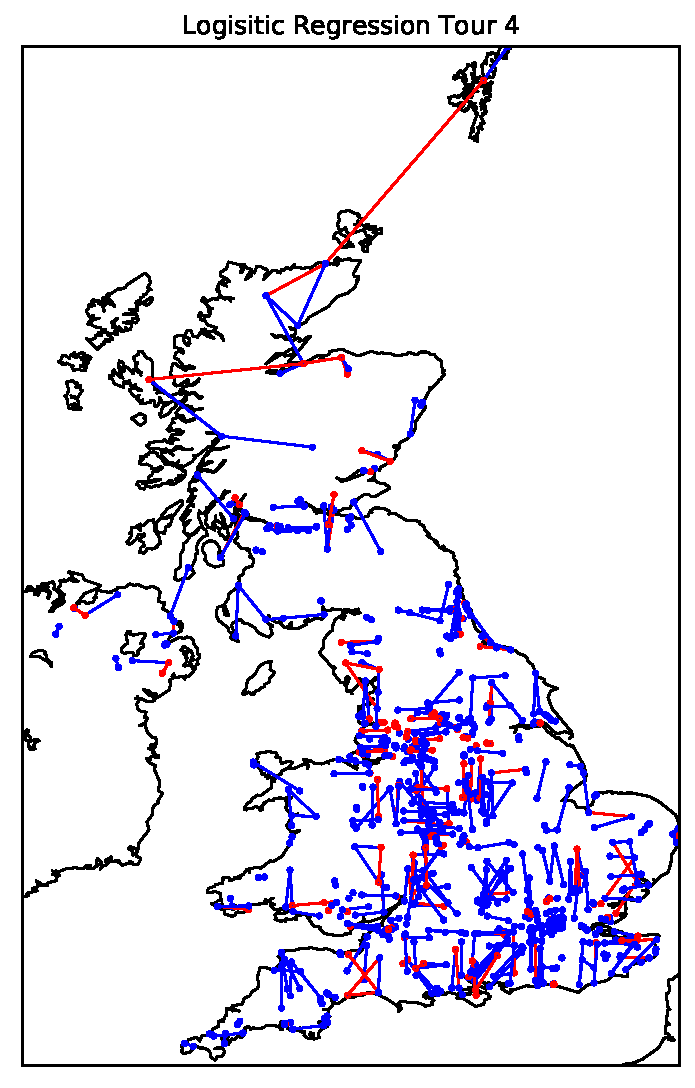
\includegraphics[width=0.4\textwidth]{Figures/map_plots/Logisitic Regression Tour 4.pdf}}
   \hfill
   \subfloat[Random Forest Predicted Edges]{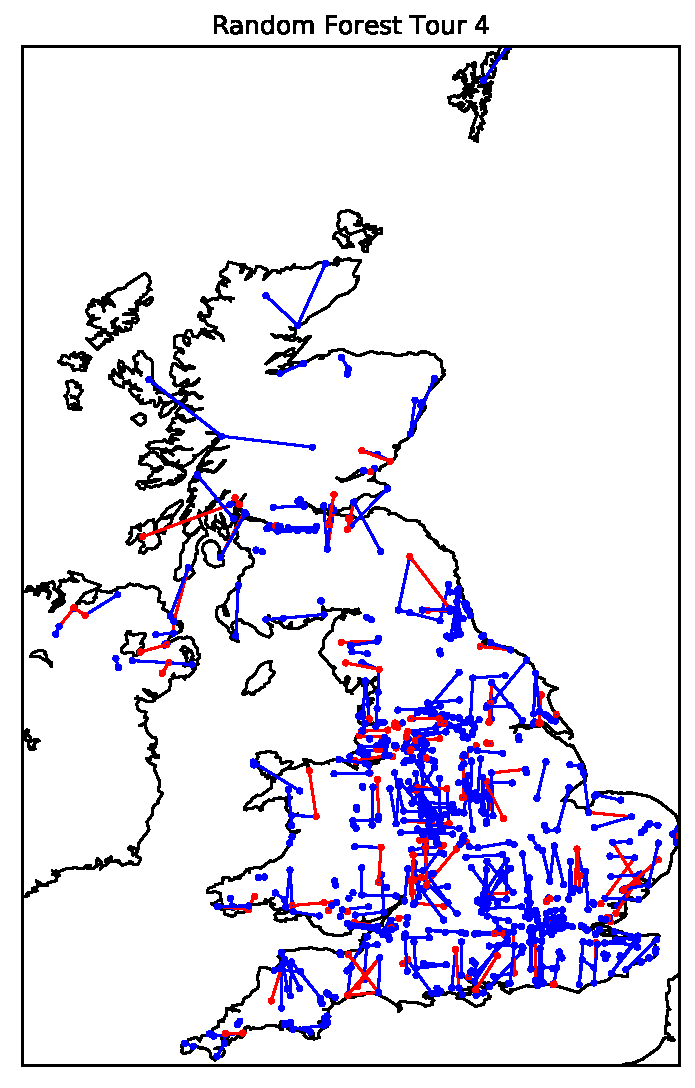
\includegraphics[width=0.4\textwidth]{Figures/map_plots/Random Forest Tour 4.pdf}}
  \caption{Concorde vs. Classifier Predicted Edges}
\end{figure}



\null\newpage
\null\newpage
\null\newpage
\null\newpage
\section{Addendum 2}\label{addendum_2}
\begin{figure}[!h]
    \centering
    \subfloat[Naïve Bayes]{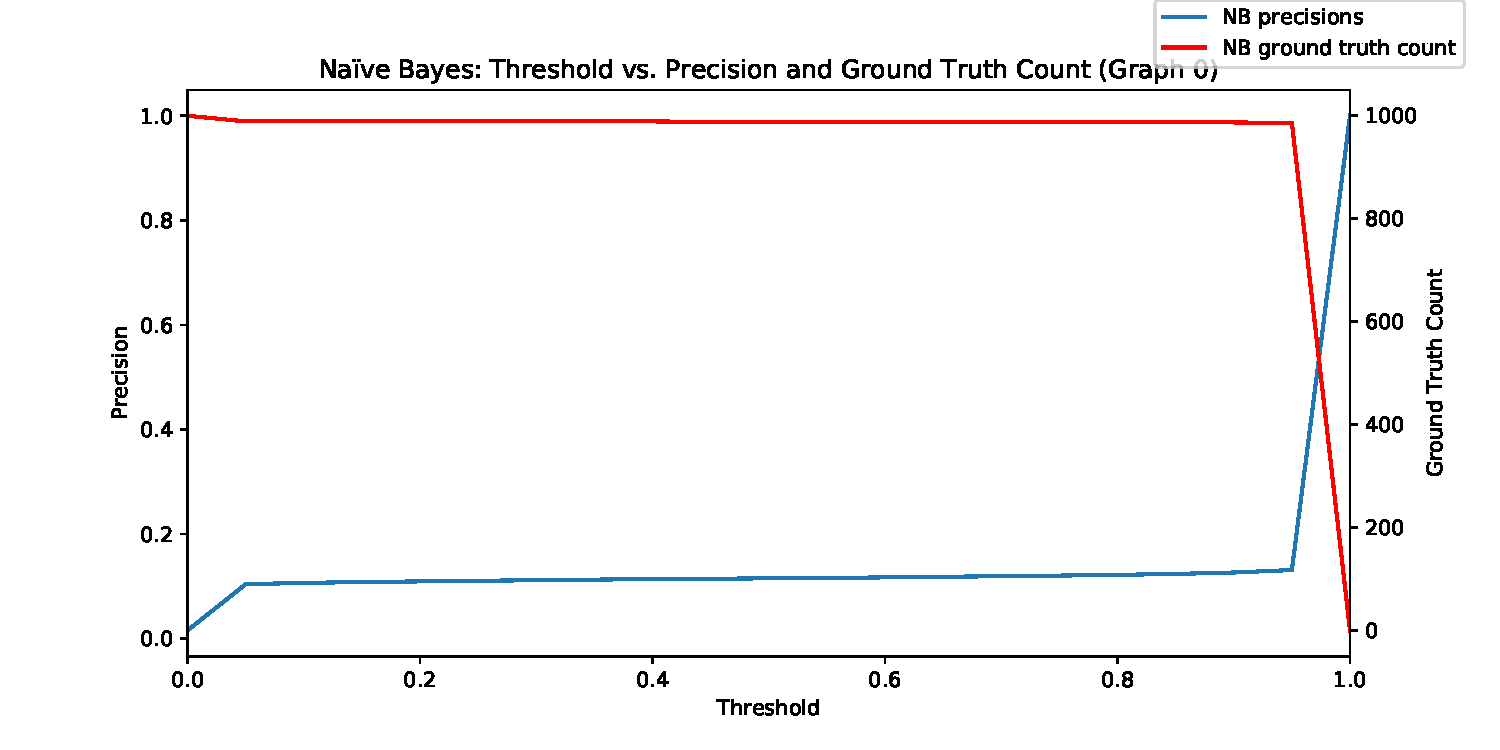
\includegraphics[width=0.8\textwidth]{Figures/exp1/NB thresh vs. precision and gtruth 0.pdf}}
    \hfill
    \subfloat[Logistic Regression]{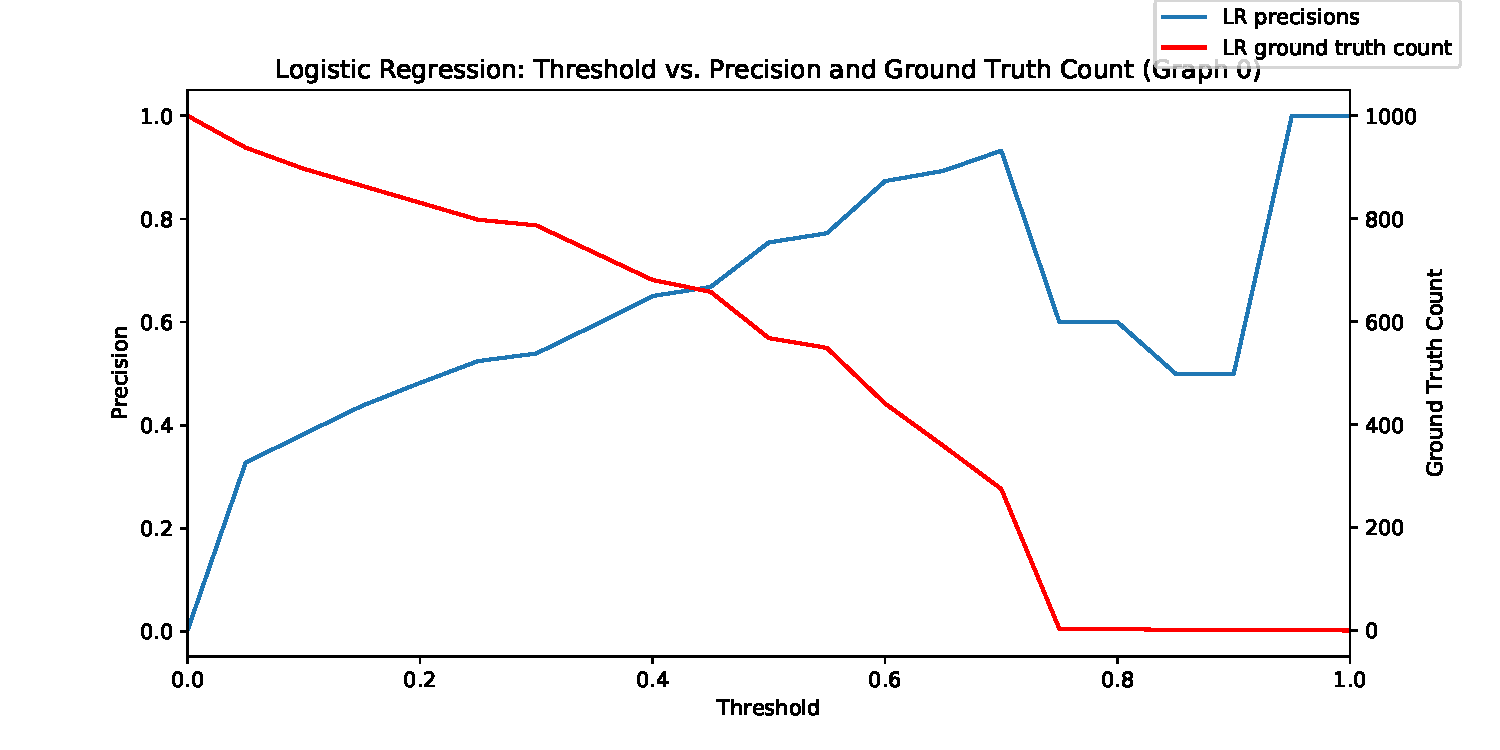
\includegraphics[width=0.8\textwidth]{Figures/exp1/LR thresh vs. precision and gtruth 0.pdf}}
    \hfill
    \subfloat[Random Forest]{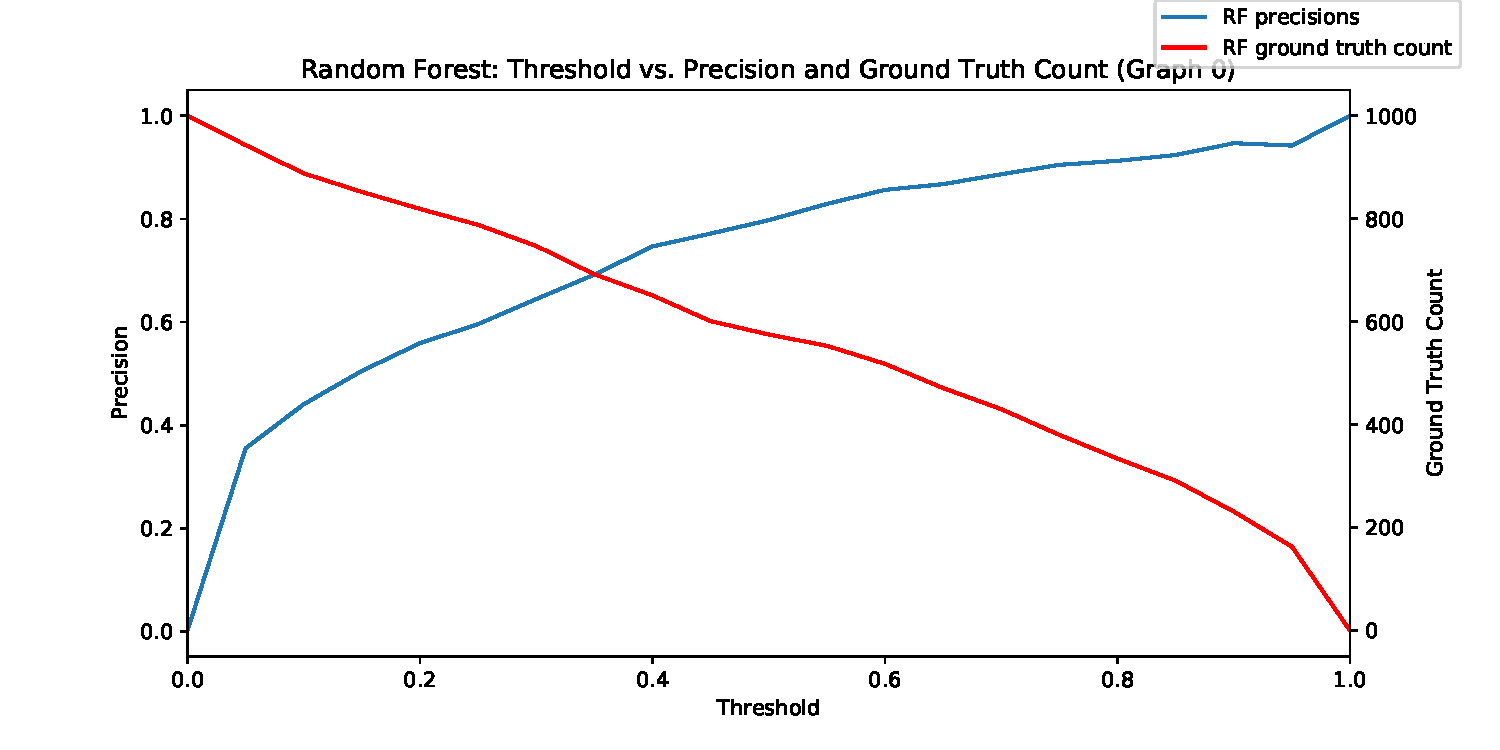
\includegraphics[width=0.8\textwidth]{Figures/exp1/RF thresh vs. precision and gtruth 0.pdf}}
    \caption{Adjusting Threshold Values}
\end{figure}

\begin{figure}[!h]
    \centering
    \subfloat[Naïve Bayes]{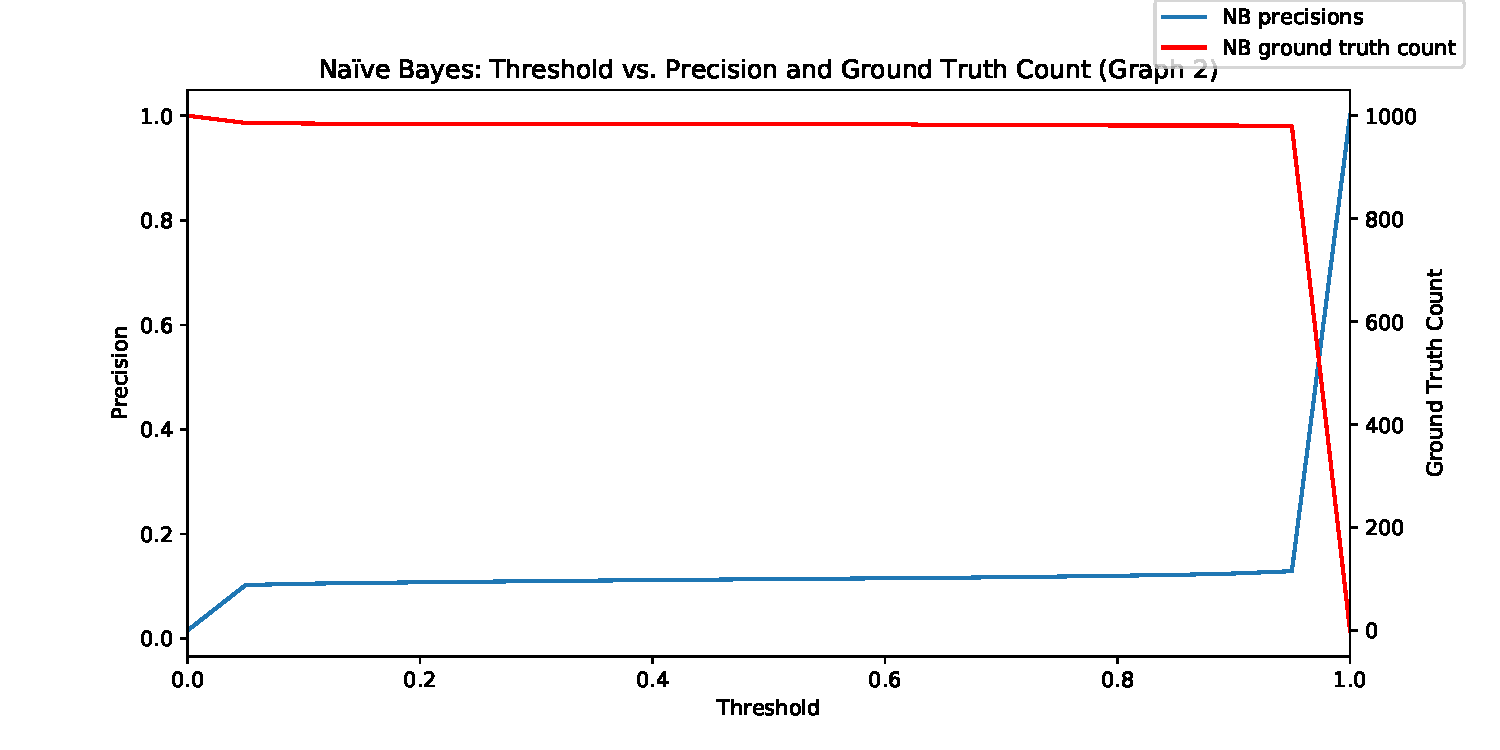
\includegraphics[width=0.8\textwidth]{Figures/exp1/NB thresh vs. precision and gtruth 2.pdf}}
    \hfill
    \subfloat[Logistic Regression]{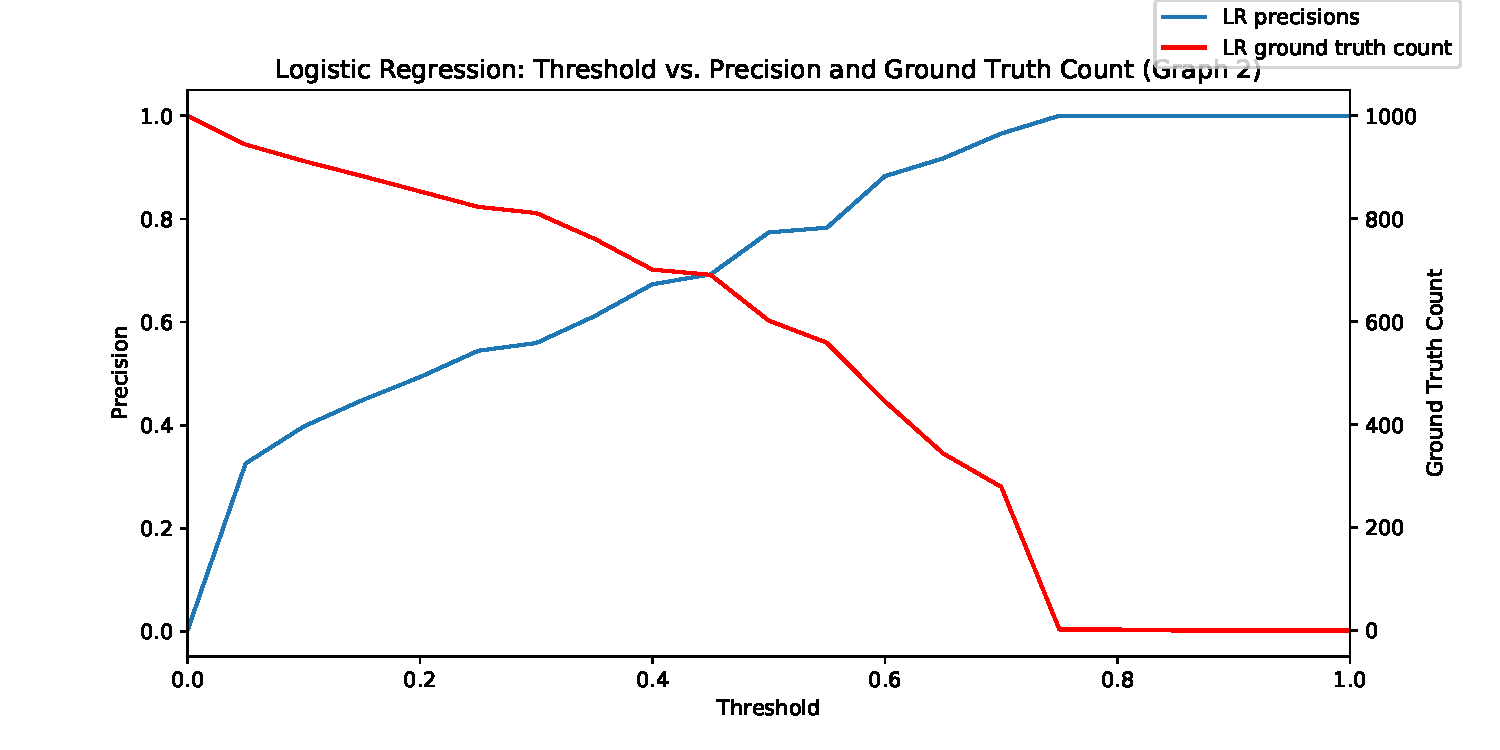
\includegraphics[width=0.8\textwidth]{Figures/exp1/LR thresh vs. precision and gtruth 2.pdf}}
    \hfill
    \subfloat[Random Forest]{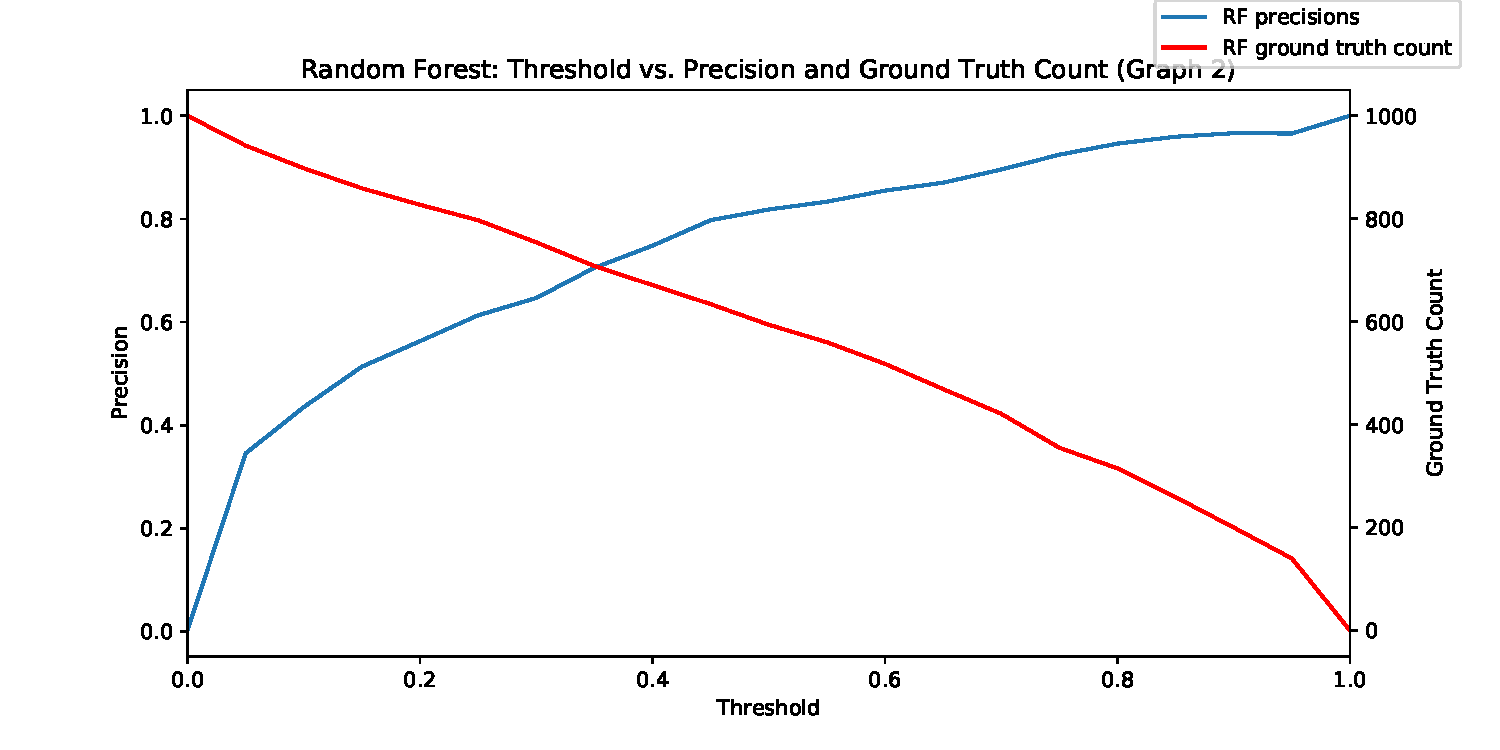
\includegraphics[width=0.8\textwidth]{Figures/exp1/RF thresh vs. precision and gtruth 2.pdf}}
    \caption{Adjusting Threshold Values}
\end{figure}

\begin{figure}[!h]
    \centering
    \subfloat[Naïve Bayes]{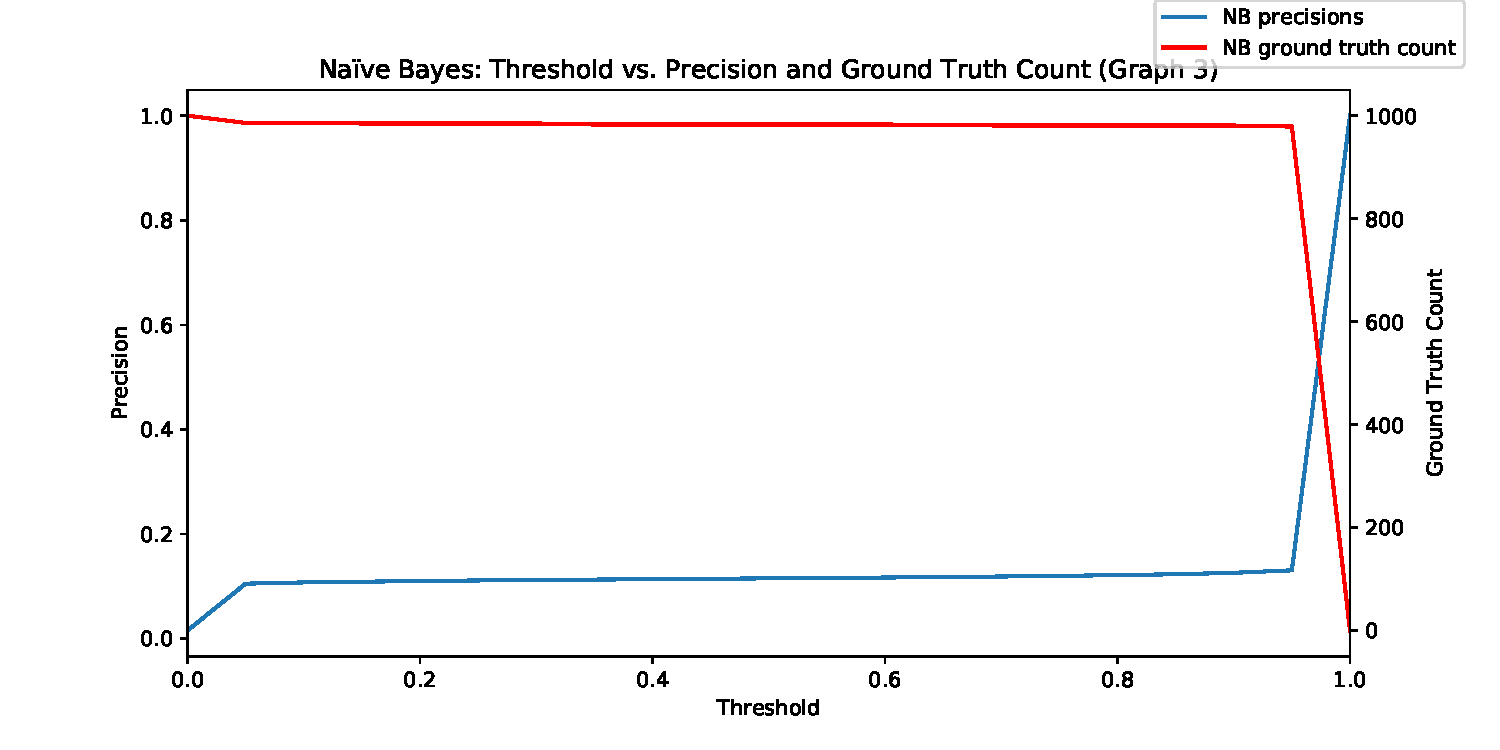
\includegraphics[width=0.8\textwidth]{Figures/exp1/NB thresh vs. precision and gtruth 3.pdf}}
    \hfill
    \subfloat[Logistic Regression]{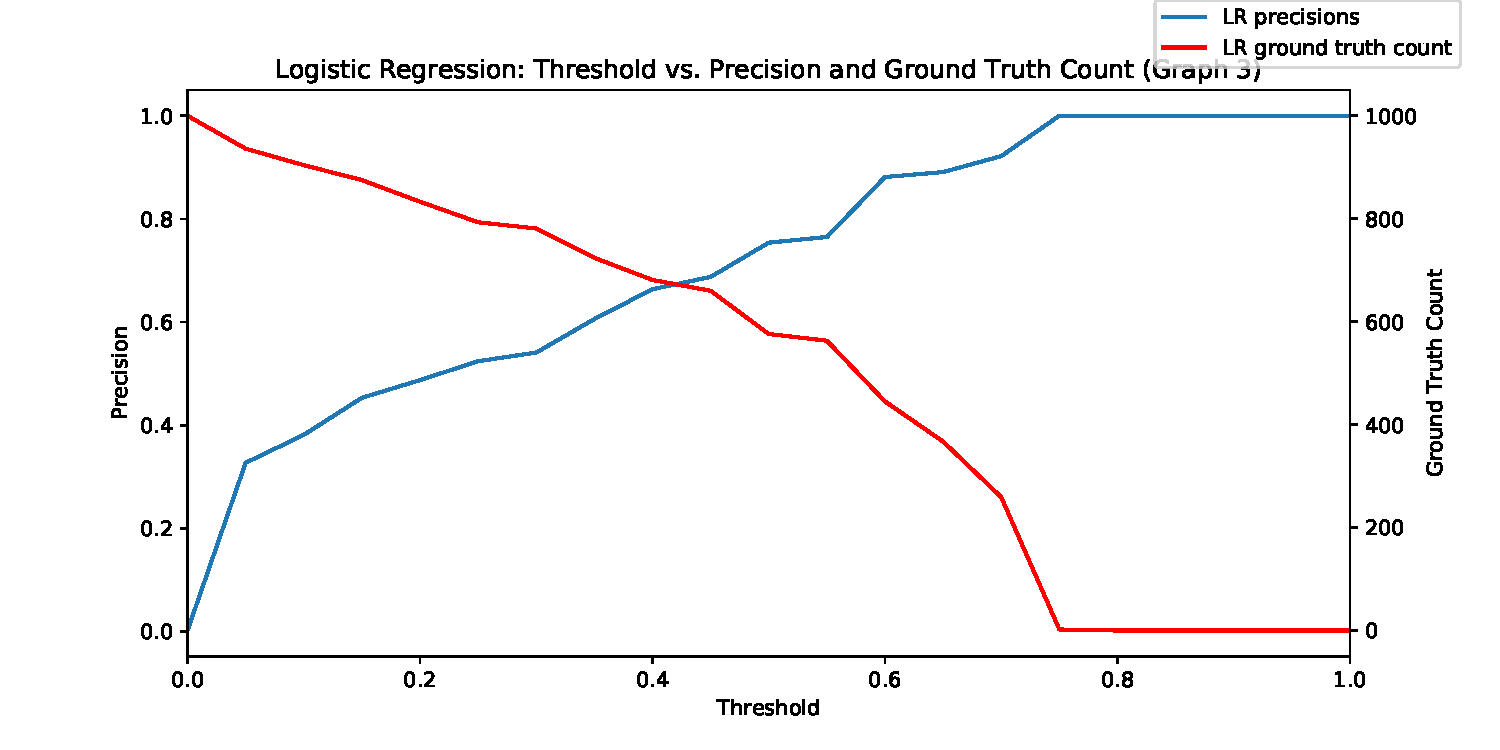
\includegraphics[width=0.8\textwidth]{Figures/exp1/LR thresh vs. precision and gtruth 3.pdf}}
    \hfill
    \subfloat[Random Forest]{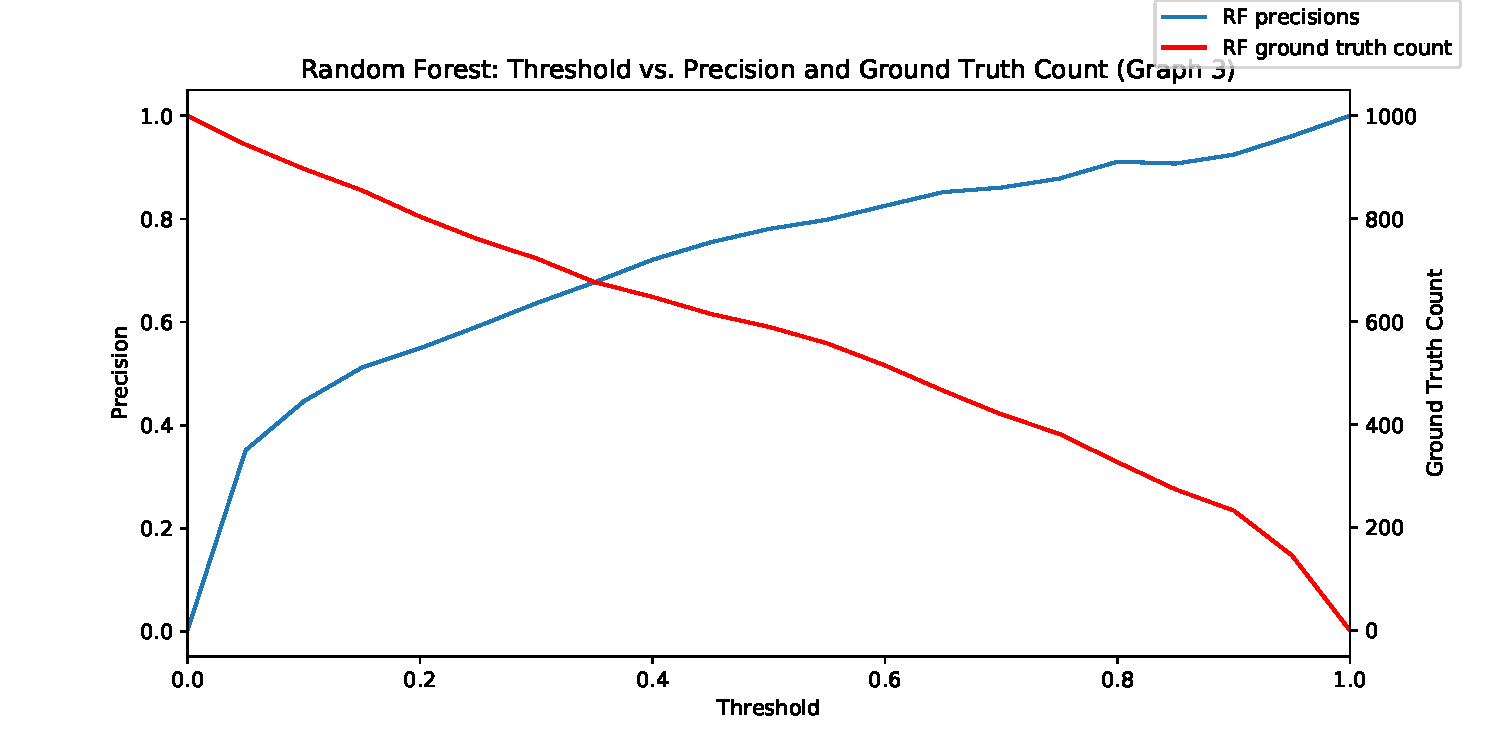
\includegraphics[width=0.8\textwidth]{Figures/exp1/RF thresh vs. precision and gtruth 3.pdf}}
    \caption{Adjusting Threshold Values}
\end{figure}

\begin{figure}[!h]
    \centering
    \subfloat[Naïve Bayes]{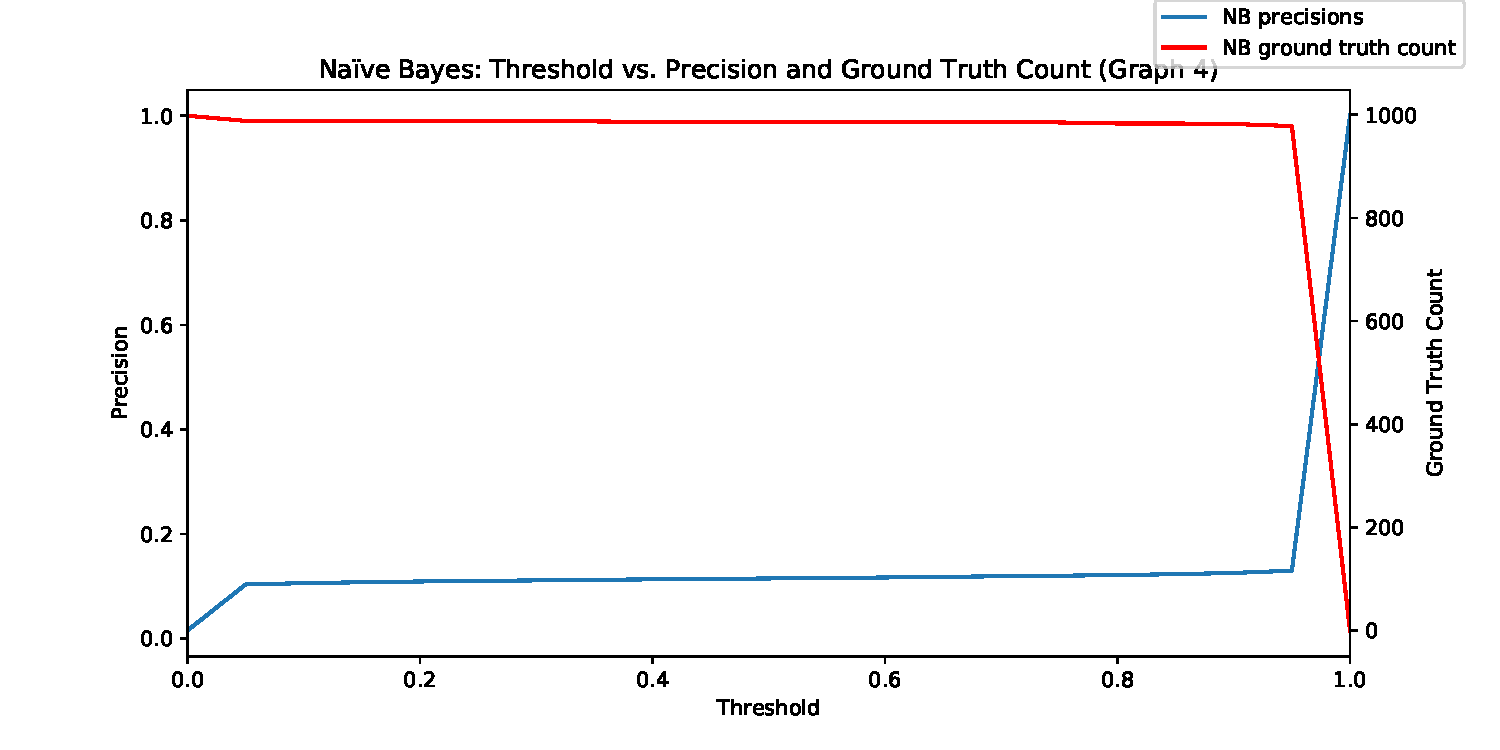
\includegraphics[width=0.8\textwidth]{Figures/exp1/NB thresh vs. precision and gtruth 4.pdf}}
    \hfill
    \subfloat[Logistic Regression]{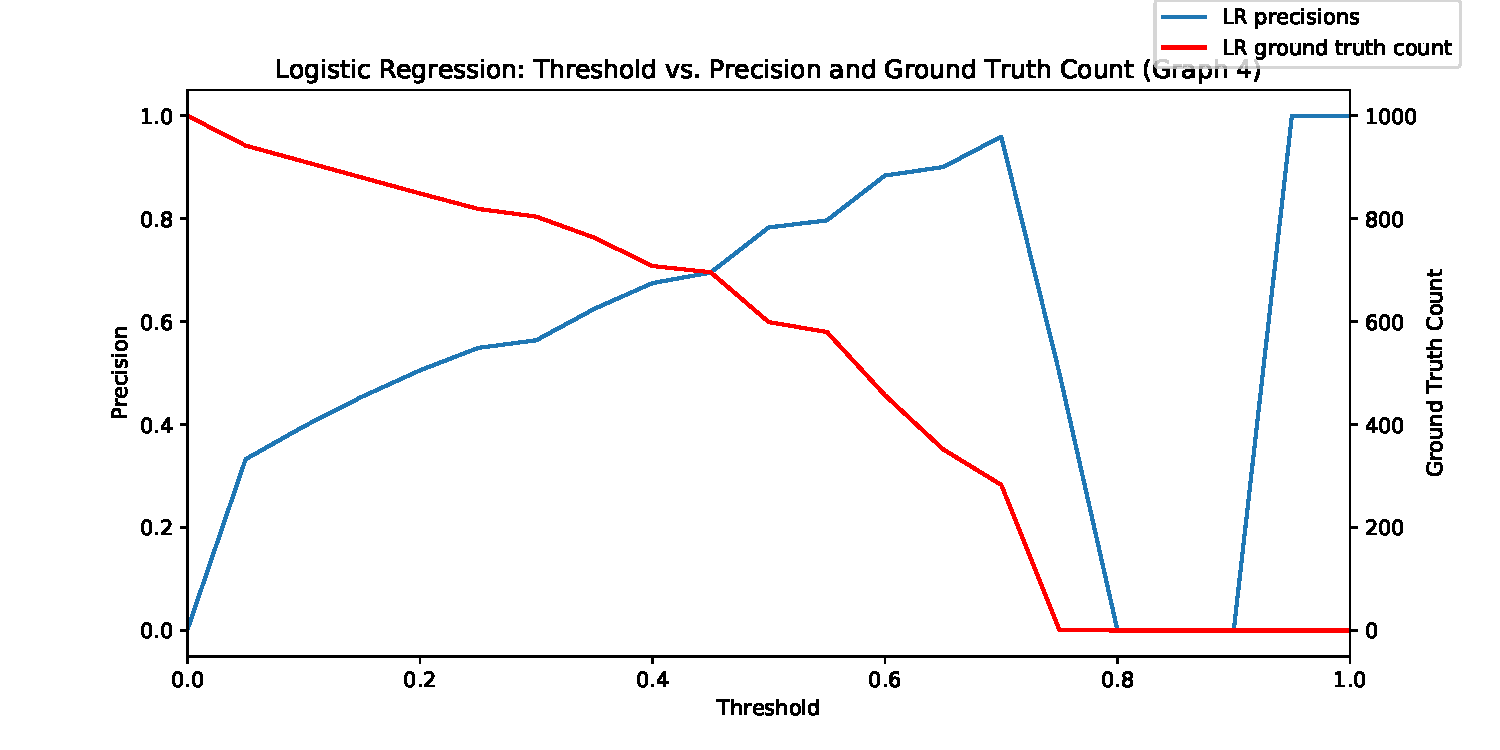
\includegraphics[width=0.8\textwidth]{Figures/exp1/LR thresh vs. precision and gtruth 4.pdf}}
    \hfill
    \subfloat[Random Forest]{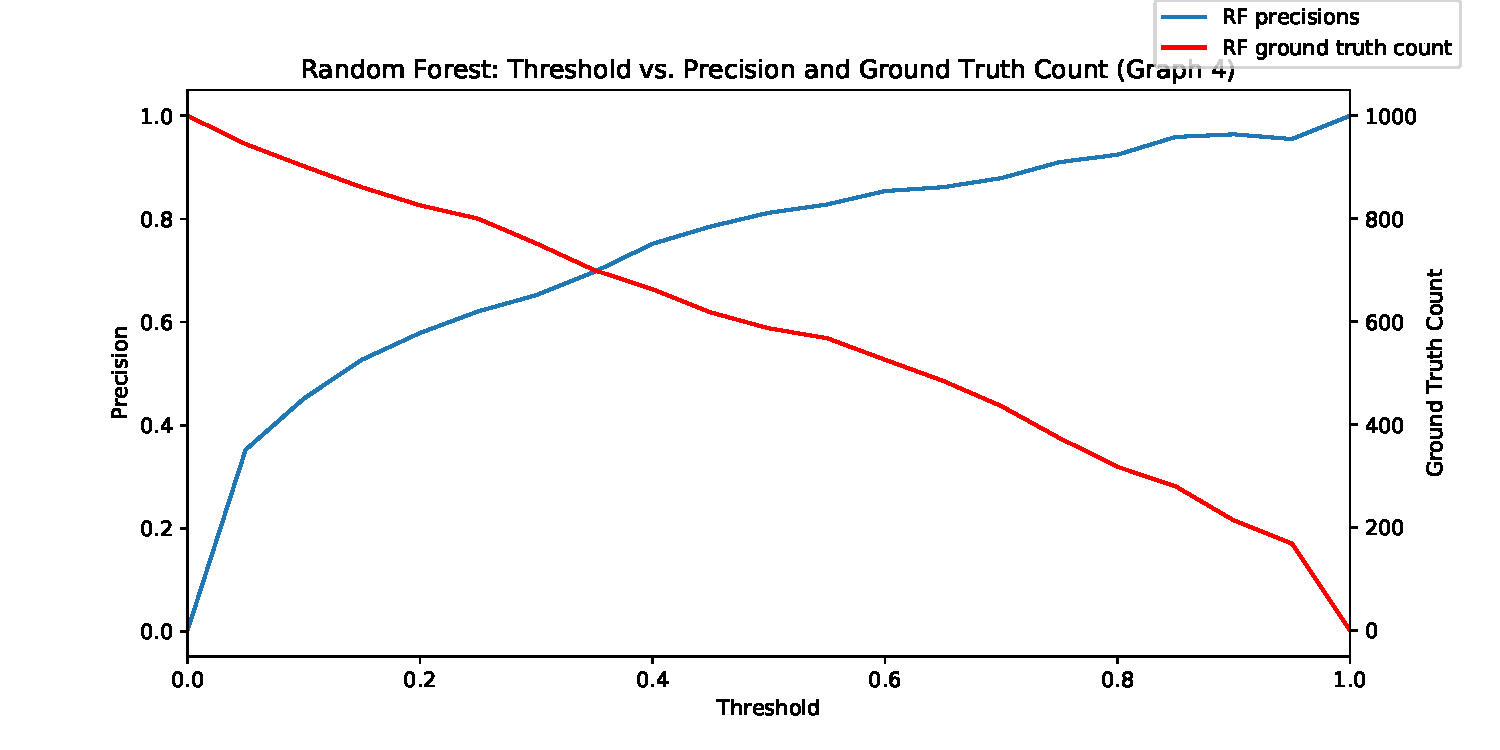
\includegraphics[width=0.8\textwidth]{Figures/exp1/RF thresh vs. precision and gtruth 4.pdf}}
    \caption{Adjusting Threshold Values}
\end{figure}

\null\newpage
\null\newpage
\null\newpage
\null\newpage
\section{Addendum 3}\label{addendum_3}
\begin{figure}[!h]
    \centering
    \subfloat[Naïve Bayes]{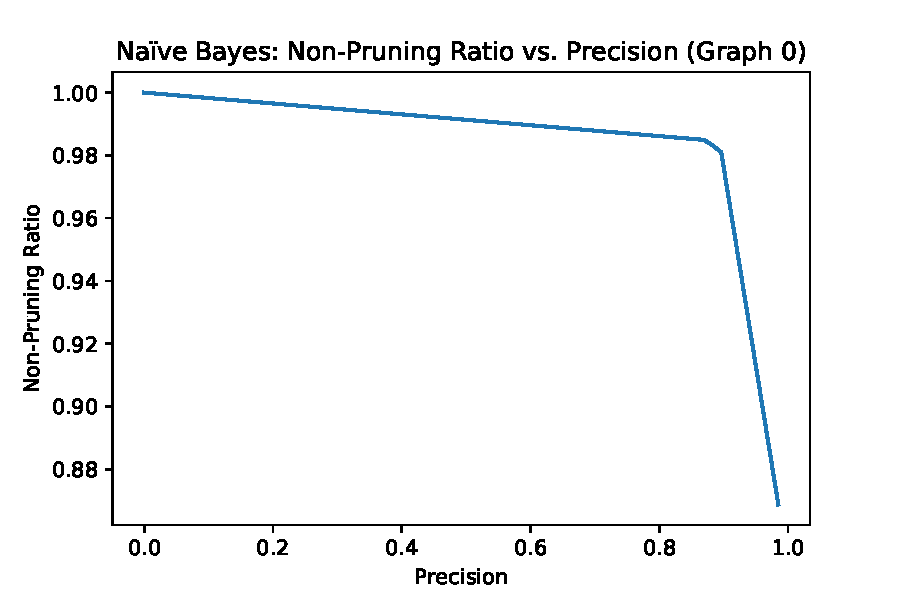
\includegraphics[width=0.6\textwidth]{Figures/exp2/NB non-prune vs precision 0.pdf}}
    \hfill
    \subfloat[Logistic Regression]{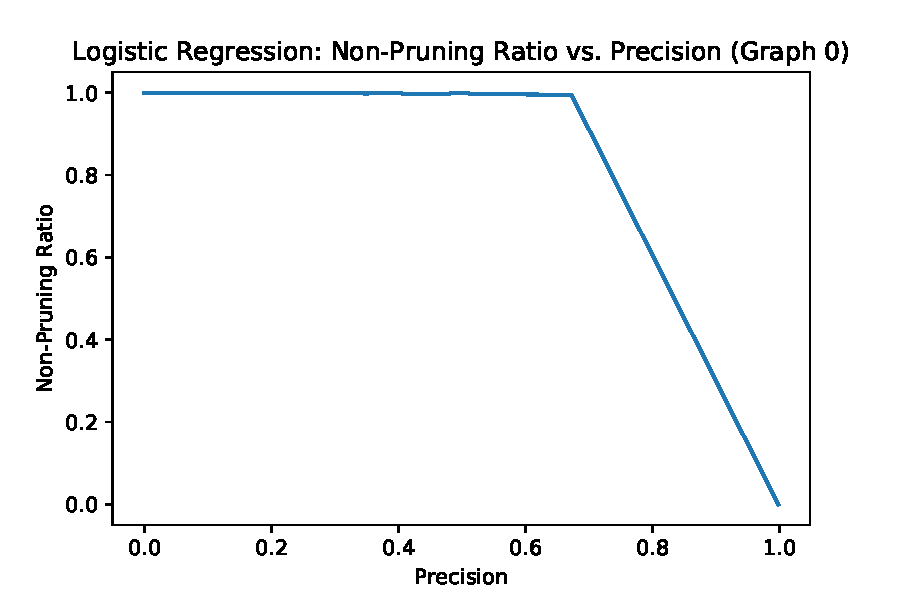
\includegraphics[width=0.6\textwidth]{Figures/exp2/LR non-prune vs precision 0.pdf}}
    \hfill
    \subfloat[Random Forest]{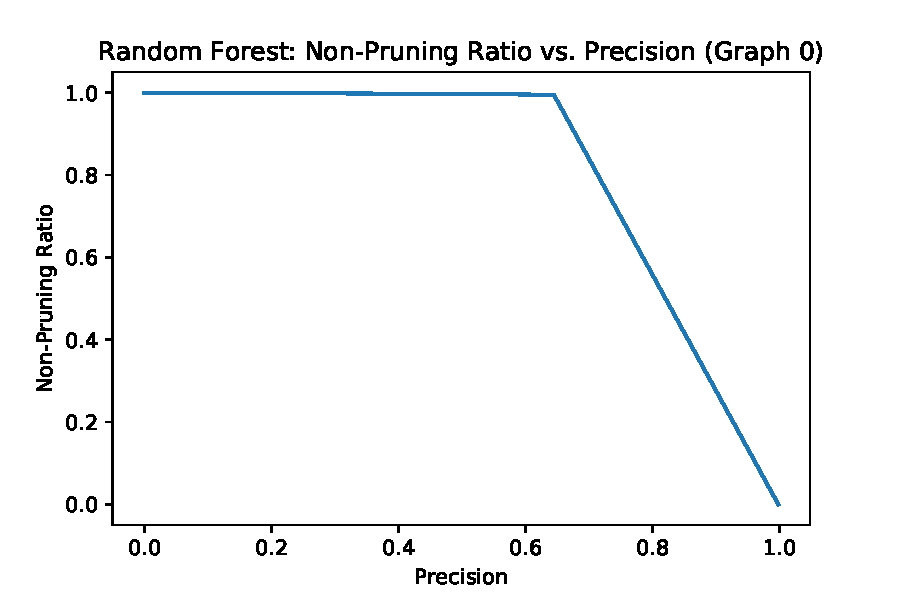
\includegraphics[width=0.6\textwidth]{Figures/exp2/RF non-prune vs precision 0.pdf}}
    \caption{Non-pruning ratio vs. Precision curve}
\end{figure}

\begin{figure}[!h]
    \centering
    \subfloat[Naïve Bayes]{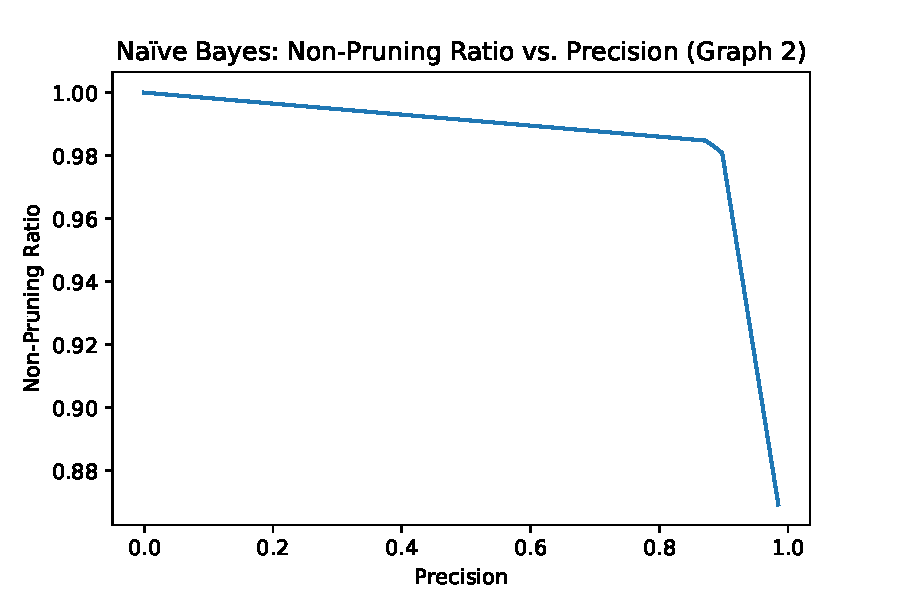
\includegraphics[width=0.7\textwidth]{Figures/exp2/NB non-prune vs precision 2.pdf}}
    \hfill
    \subfloat[Logistic Regression]{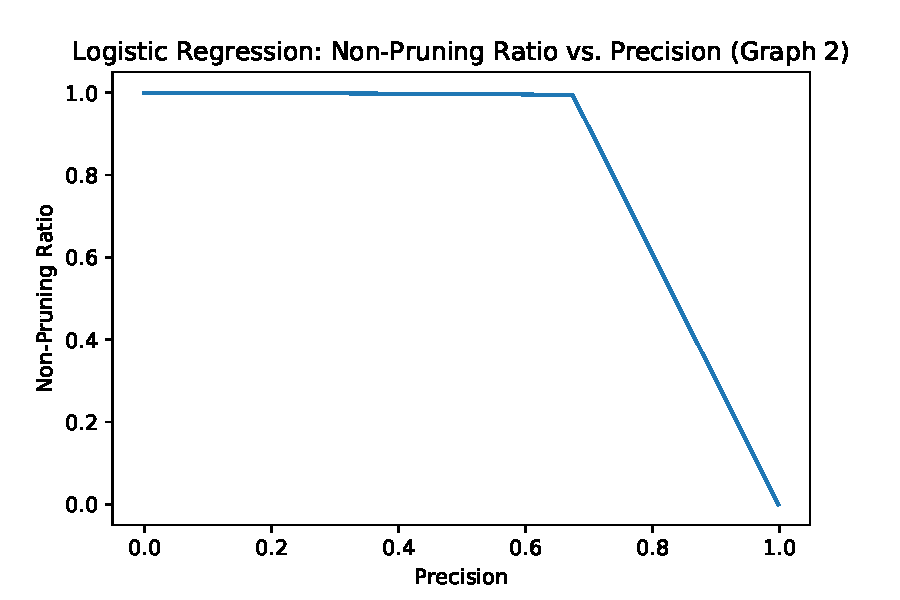
\includegraphics[width=0.7\textwidth]{Figures/exp2/LR non-prune vs precision 2.pdf}}
    \hfill
    \subfloat[Random Forest]{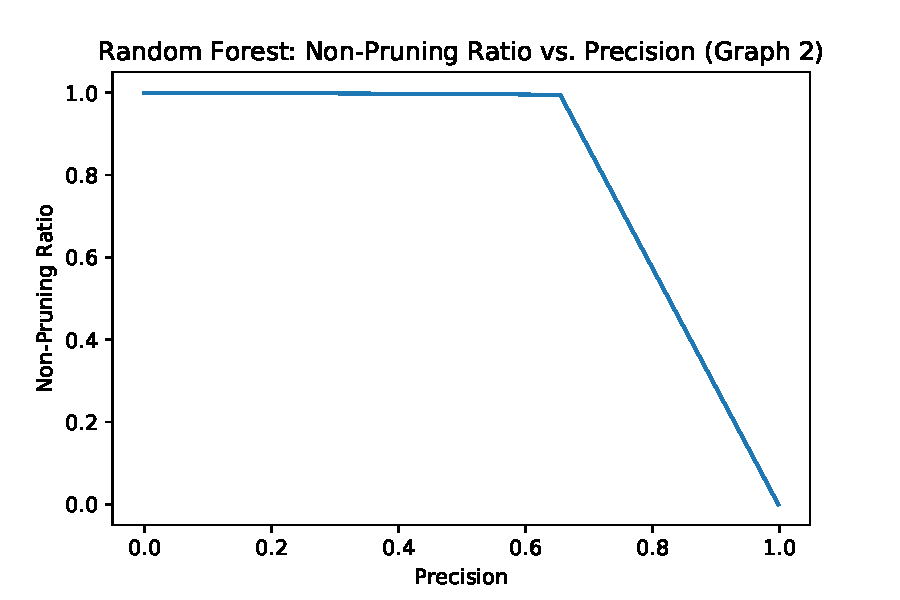
\includegraphics[width=0.7\textwidth]{Figures/exp2/RF non-prune vs precision 2.pdf}}
    \caption{Non-pruning ratio vs. Precision curve}
\end{figure}

\begin{figure}[!h]
    \centering
    \subfloat[Naïve Bayes]{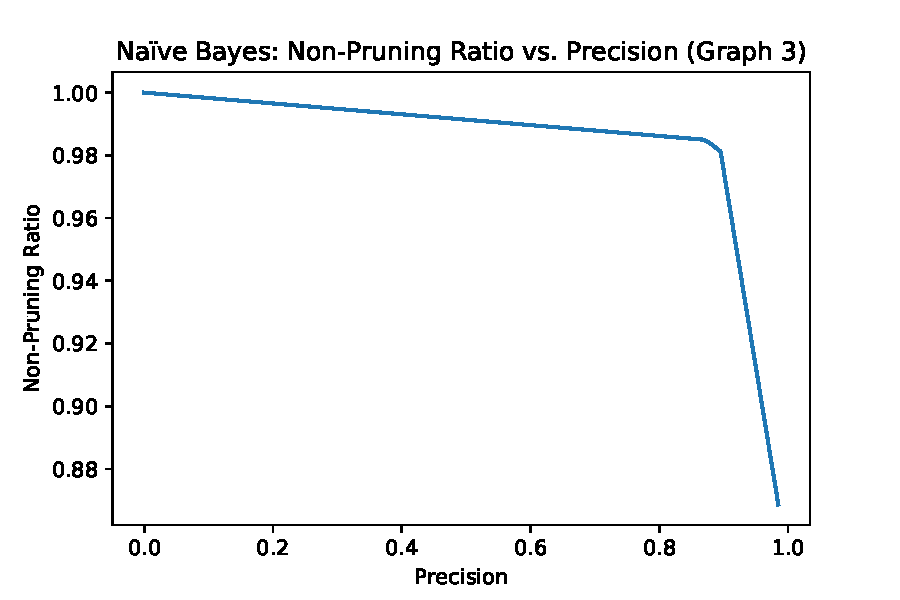
\includegraphics[width=0.7\textwidth]{Figures/exp2/NB non-prune vs precision 3.pdf}}
    \hfill
    \subfloat[Logistic Regression]{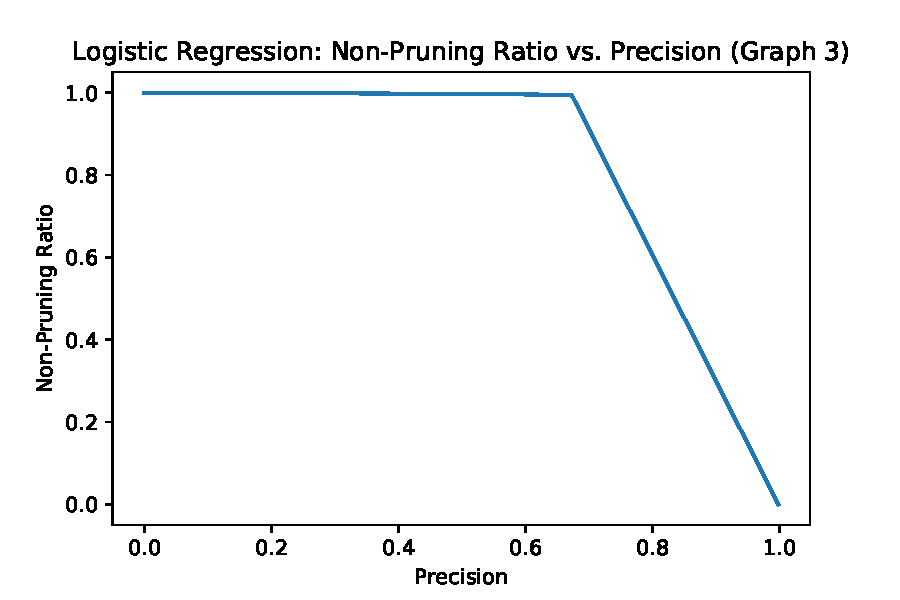
\includegraphics[width=0.7\textwidth]{Figures/exp2/LR non-prune vs precision 3.pdf}}
    \hfill
    \subfloat[Random Forest]{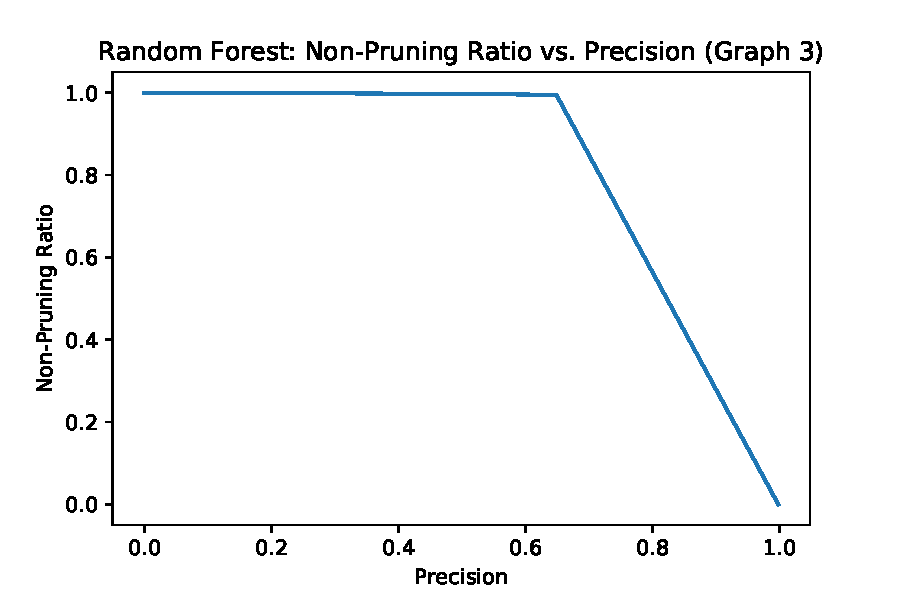
\includegraphics[width=0.7\textwidth]{Figures/exp2/RF non-prune vs precision 3.pdf}}
    \caption{Non-pruning ratio vs. Precision curve}
\end{figure}

\begin{figure}[!h]
    \centering
    \subfloat[Naïve Bayes]{\includegraphics[width=0.7\textwidth]{Figures/exp2/NB non-prune vs precision 4.pdf}}
    \hfill
    \subfloat[Logistic Regression]{\includegraphics[width=0.7\textwidth]{Figures/exp2/LR non-prune vs precision 4.pdf}}
    \hfill
    \subfloat[Random Forest]{\includegraphics[width=0.7\textwidth]{Figures/exp2/RF non-prune vs precision 4.pdf}}
    \caption{Non-pruning ratio vs. Precision curve}
\end{figure}

%%%% ADD YOUR BIBLIOGRAPHY HERE
\printbibliography

%%%%
%%%% maybe code listing here?

%%%%
\end{document}
%\end{article}